%%%%%%%%%1%%%%%%%%%2%%%%%%%%%3%%%%%%%%%4%%%%%%%%%5%%%%%%%%%6%%%%%%%%%7%%%%%%%%%8
% Beamer Header
%%%%%%%%%1%%%%%%%%%2%%%%%%%%%3%%%%%%%%%4%%%%%%%%%5%%%%%%%%%6%%%%%%%%%7%%%%%%%%%8

\documentclass[compress,english]{beamer}
\usetheme{sthlm}

% Basic beamer packages
\usepackage{booktabs}
\usepackage{datetime}
\usepackage{dtklogos}
\usepackage{graphicx}
\usepackage{multicol}
\usepackage{pgfplots}
\usepackage{ragged2e}
\usepackage{tabularx}
\usepackage{tikz}
\usepackage{wasysym}

\pgfplotsset{compat=1.8}

\usepackage[utf8]{inputenc}
\usepackage[T1]{fontenc}
\usepackage{newpxtext,newpxmath}

% tikz
\usepackage{tikz}
\usetikzlibrary{patterns,backgrounds,mindmap}

% additional packages
\usepackage{listings}
\usepackage{units}
\usepackage{babel}
\usepackage{sansmath}

\makeatother

%%%%%%%%%1%%%%%%%%%2%%%%%%%%%3%%%%%%%%%4%%%%%%%%%5%%%%%%%%%6%%%%%%%%%7%%%%%%%%%8
% Graphics Path
%%%%%%%%%1%%%%%%%%%2%%%%%%%%%3%%%%%%%%%4%%%%%%%%%5%%%%%%%%%6%%%%%%%%%7%%%%%%%%%8

\graphicspath{{images/}{../images/}}

%%%%%%%%%1%%%%%%%%%2%%%%%%%%%3%%%%%%%%%4%%%%%%%%%5%%%%%%%%%6%%%%%%%%%7%%%%%%%%%8
% Footnote rule
%%%%%%%%%1%%%%%%%%%2%%%%%%%%%3%%%%%%%%%4%%%%%%%%%5%%%%%%%%%6%%%%%%%%%7%%%%%%%%%8

\renewcommand{\footnoterule}{%
}

%%%%%%%%%1%%%%%%%%%2%%%%%%%%%3%%%%%%%%%4%%%%%%%%%5%%%%%%%%%6%%%%%%%%%7%%%%%%%%%8
% Default Background Image
%%%%%%%%%1%%%%%%%%%2%%%%%%%%%3%%%%%%%%%4%%%%%%%%%5%%%%%%%%%6%%%%%%%%%7%%%%%%%%%8

%\usebackgroundtemplate%
%	{\includegraphics[width=\paperwidth,height=\paperheight]{background2.png}}

%%%%%%%%%1%%%%%%%%%2%%%%%%%%%3%%%%%%%%%4%%%%%%%%%5%%%%%%%%%6%%%%%%%%%7%%%%%%%%%8
% Presentation Information
%%%%%%%%%1%%%%%%%%%2%%%%%%%%%3%%%%%%%%%4%%%%%%%%%5%%%%%%%%%6%%%%%%%%%7%%%%%%%%%8

\title{\vspace{20pt}Research Overview: Controlling Water Levels on the Rainy Lake/Namakan Reservoir System.}
\author{Jeff Kantor}
\institute{University of Notre Dame \\ Github: \href{http://jckantor.github.io/Rainy-Lake-Hydrology/}{http://jckantor.github.io/Rainy-Lake-Hydrology/}}
\subtitle{$\ $}
\date{September, 2015}

\begin{document}

%%%%%%%%%1%%%%%%%%%2%%%%%%%%%3%%%%%%%%%4%%%%%%%%%5%%%%%%%%%6%%%%%%%%%7%%%%%%%%%8
% Title Page
%%%%%%%%%1%%%%%%%%%2%%%%%%%%%3%%%%%%%%%4%%%%%%%%%5%%%%%%%%%6%%%%%%%%%7%%%%%%%%%8

\setbeamercolor{title}{fg=red}
\setbeamercolor{subtitle}{fg=white}
\setbeamercolor{date}{fg=white}
\setbeamercolor{author}{fg=white}
\setbeamercolor{institute}{fg=white}

\setbeamerfont{title}{series=\bfseries}

{\usebackgroundtemplate%
	{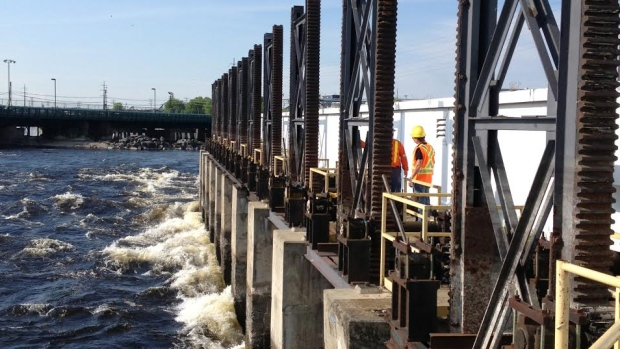
\includegraphics[height=\paperheight]{fort-frances-dam.jpg}}

\begin{frame}[plain]
\titlepage
\end{frame}
}

%%%%%%%%%1%%%%%%%%%2%%%%%%%%%3%%%%%%%%%4%%%%%%%%%5%%%%%%%%%6%%%%%%%%%7%%%%%%%%%8
\begin{frame}{Rainy Lake/Namakan Reservoir}

\begin{center}
\includegraphicscopyright[height=0.75\paperheight]{1029px-USA_Minnesota_location_map.png}{Source: \href{https://en.wikipedia.org/wiki/Rainy_Lake}{Wikimedia Commons}}
\end{center}

\end{frame}

%%%%%%%%%1%%%%%%%%%2%%%%%%%%%3%%%%%%%%%4%%%%%%%%%5%%%%%%%%%6%%%%%%%%%7%%%%%%%%%8
\begin{frame}{Canadian Shield}

\begin{center}
\includegraphicscopyright[height=0.6\paperheight]{Canada_geological_map}{Source: \href{https://en.wikipedia.org/wiki/Rainy_Lake}{Wikimedia Commons}}
\end{center}
\begin{itemize}
\item Estimates range from 8\% to 20\% of world's fresh water.
\item Average lake water conductivity of 19 $\frac{\mu S}{cm}$, very poorly buffered.
\item 250,000 lakes in Ontario.

\end{itemize}
\vfill
\end{frame}

%%%%%%%%%1%%%%%%%%%2%%%%%%%%%3%%%%%%%%%4%%%%%%%%%5%%%%%%%%%6%%%%%%%%%7%%%%%%%%%8
\begin{frame}{Major River Basins of the World}

\begin{center}
\includegraphicscopyright[height=0.8\paperheight]{0201-majorbasins-EN.jpg}{Source: \href{http://www.unep.org/dewa/vitalwater/article34.html}{UNEP Vital Water Graphics}}
\end{center}
\end{frame}

%%%%%%%%%1%%%%%%%%%2%%%%%%%%%3%%%%%%%%%4%%%%%%%%%5%%%%%%%%%6%%%%%%%%%7%%%%%%%%%8

{{\usebackgroundtemplate%
	{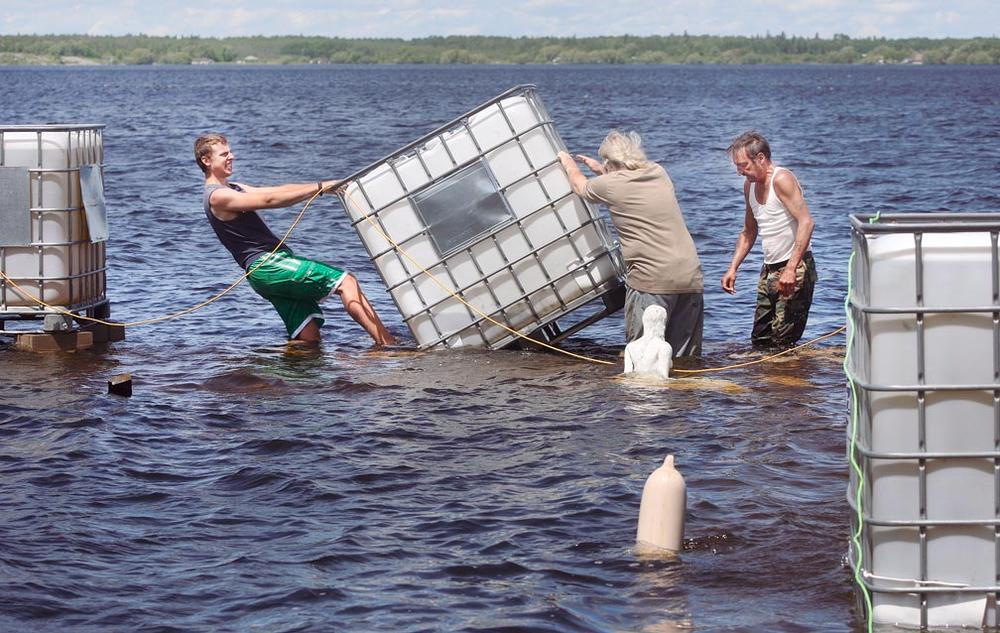
\includegraphics[height=\paperheight]{kingFLOOD0617c4.jpg}}

\begin{frame}{Summer Flooding 2014}

\footnotetext{\color{white}{Photo by Bob King (rking@duluthnews.com)}}

\end{frame}
}

%%%%%%%%%1%%%%%%%%%2%%%%%%%%%3%%%%%%%%%4%%%%%%%%%5%%%%%%%%%6%%%%%%%%%7%%%%%%%%%8

{{\usebackgroundtemplate%
	{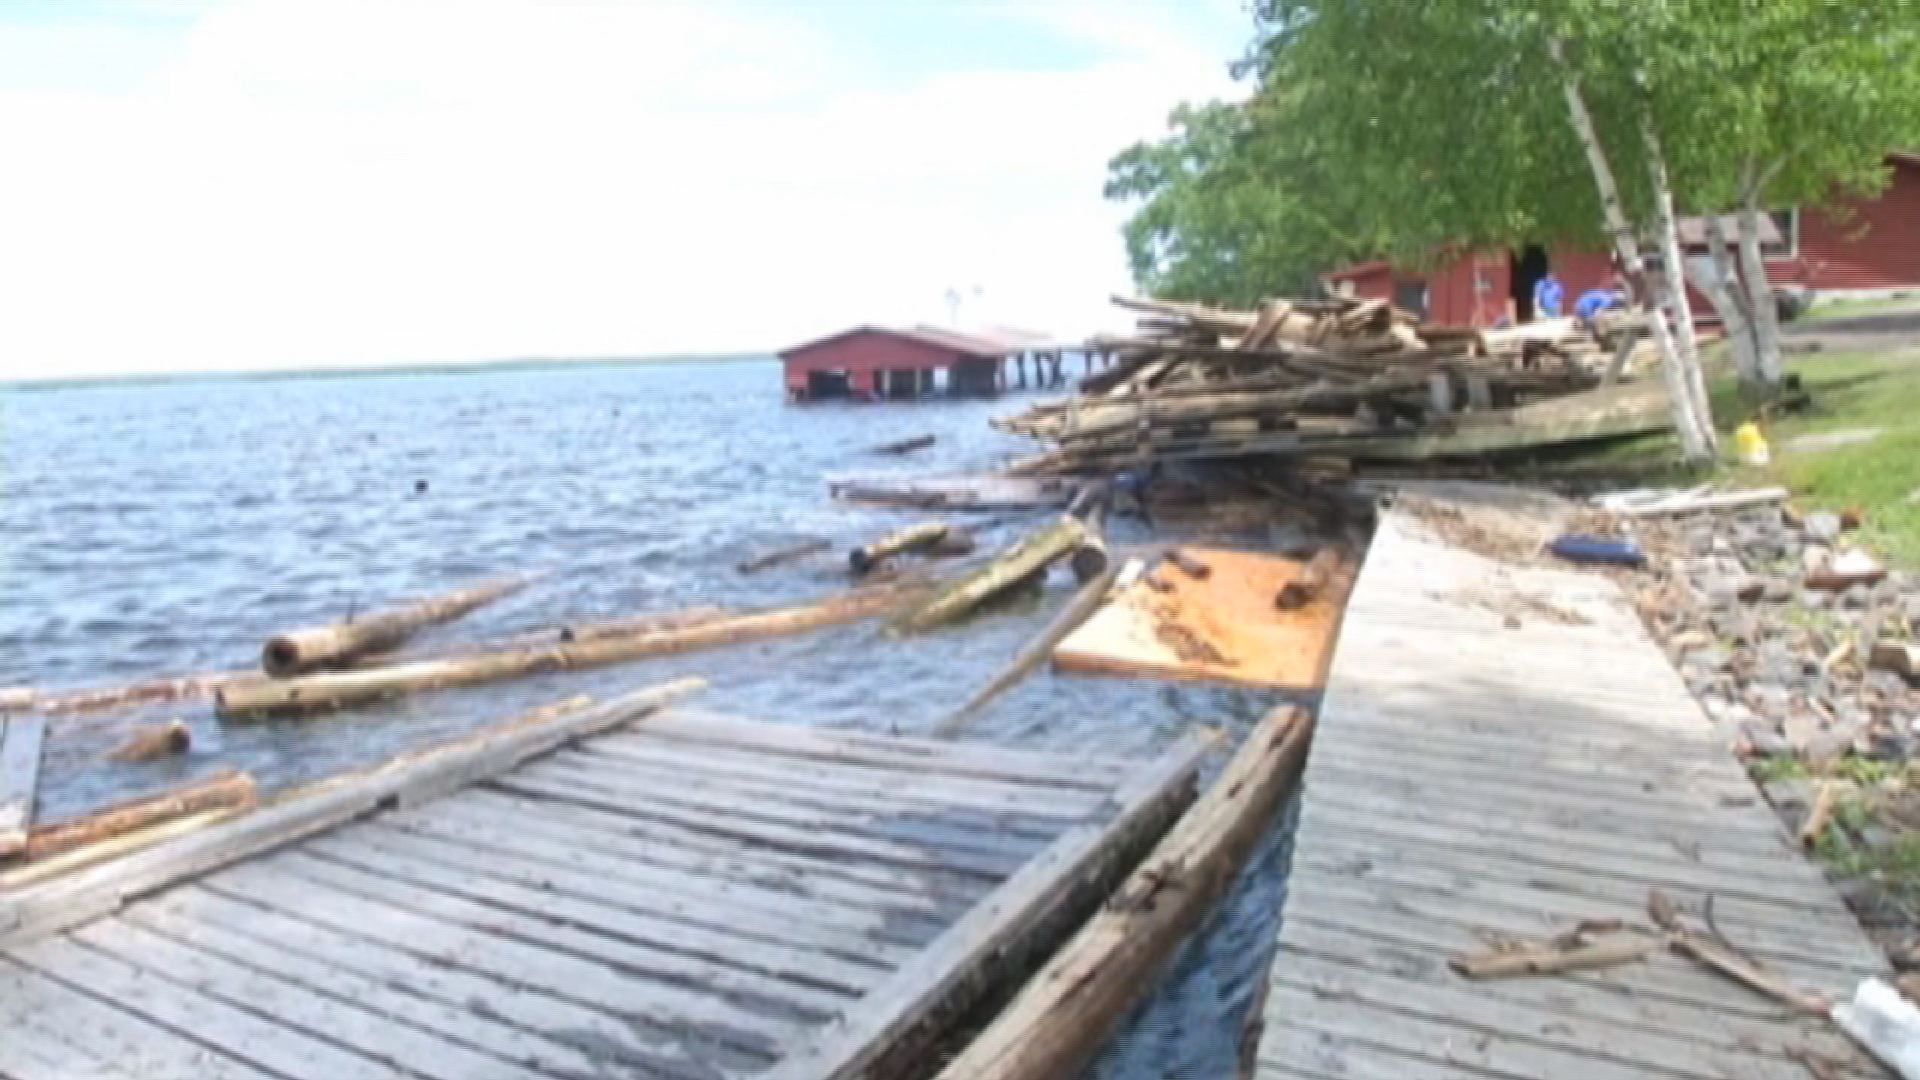
\includegraphics[height=\paperheight]{resort-damage-2.jpg}}

\begin{frame}{}

\footnotetext{\color{white}{Photo by WCCO, CBS Minnesota}}
  
\end{frame}
}

%%%%%%%%%1%%%%%%%%%2%%%%%%%%%3%%%%%%%%%4%%%%%%%%%5%%%%%%%%%6%%%%%%%%%7%%%%%%%%%8

{{\usebackgroundtemplate%
	{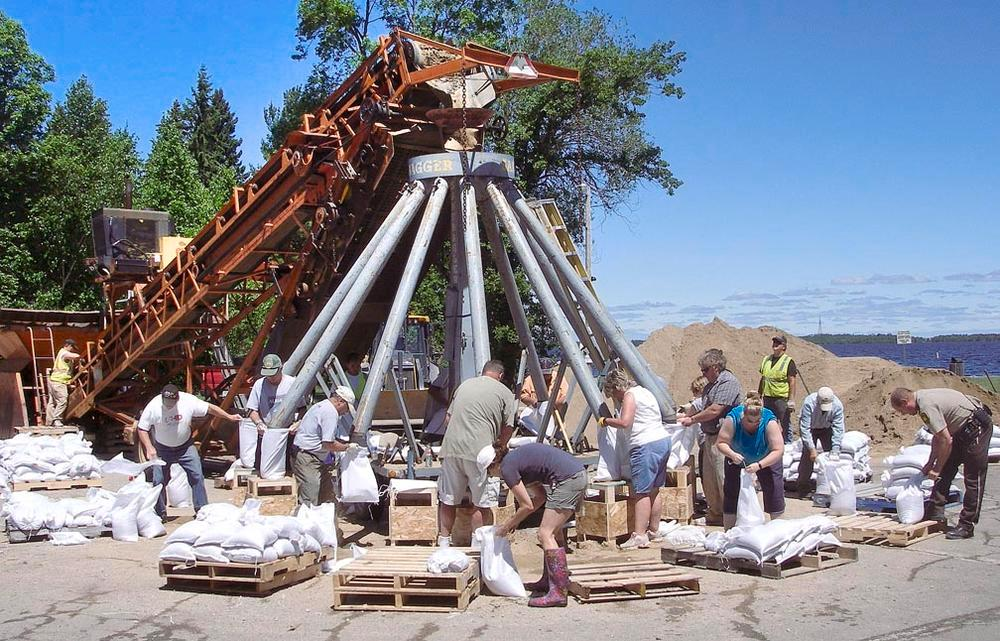
\includegraphics[height=\paperheight]{myersFLOOD0618c10_0.jpg}}

\begin{frame}{}

\footnotetext{\color{white}{Photo by John Meyers, Duluth News Tribune}}
  
\end{frame}
}

%%%%%%%%%1%%%%%%%%%2%%%%%%%%%3%%%%%%%%%4%%%%%%%%%5%%%%%%%%%6%%%%%%%%%7%%%%%%%%%8

{{\usebackgroundtemplate%
	{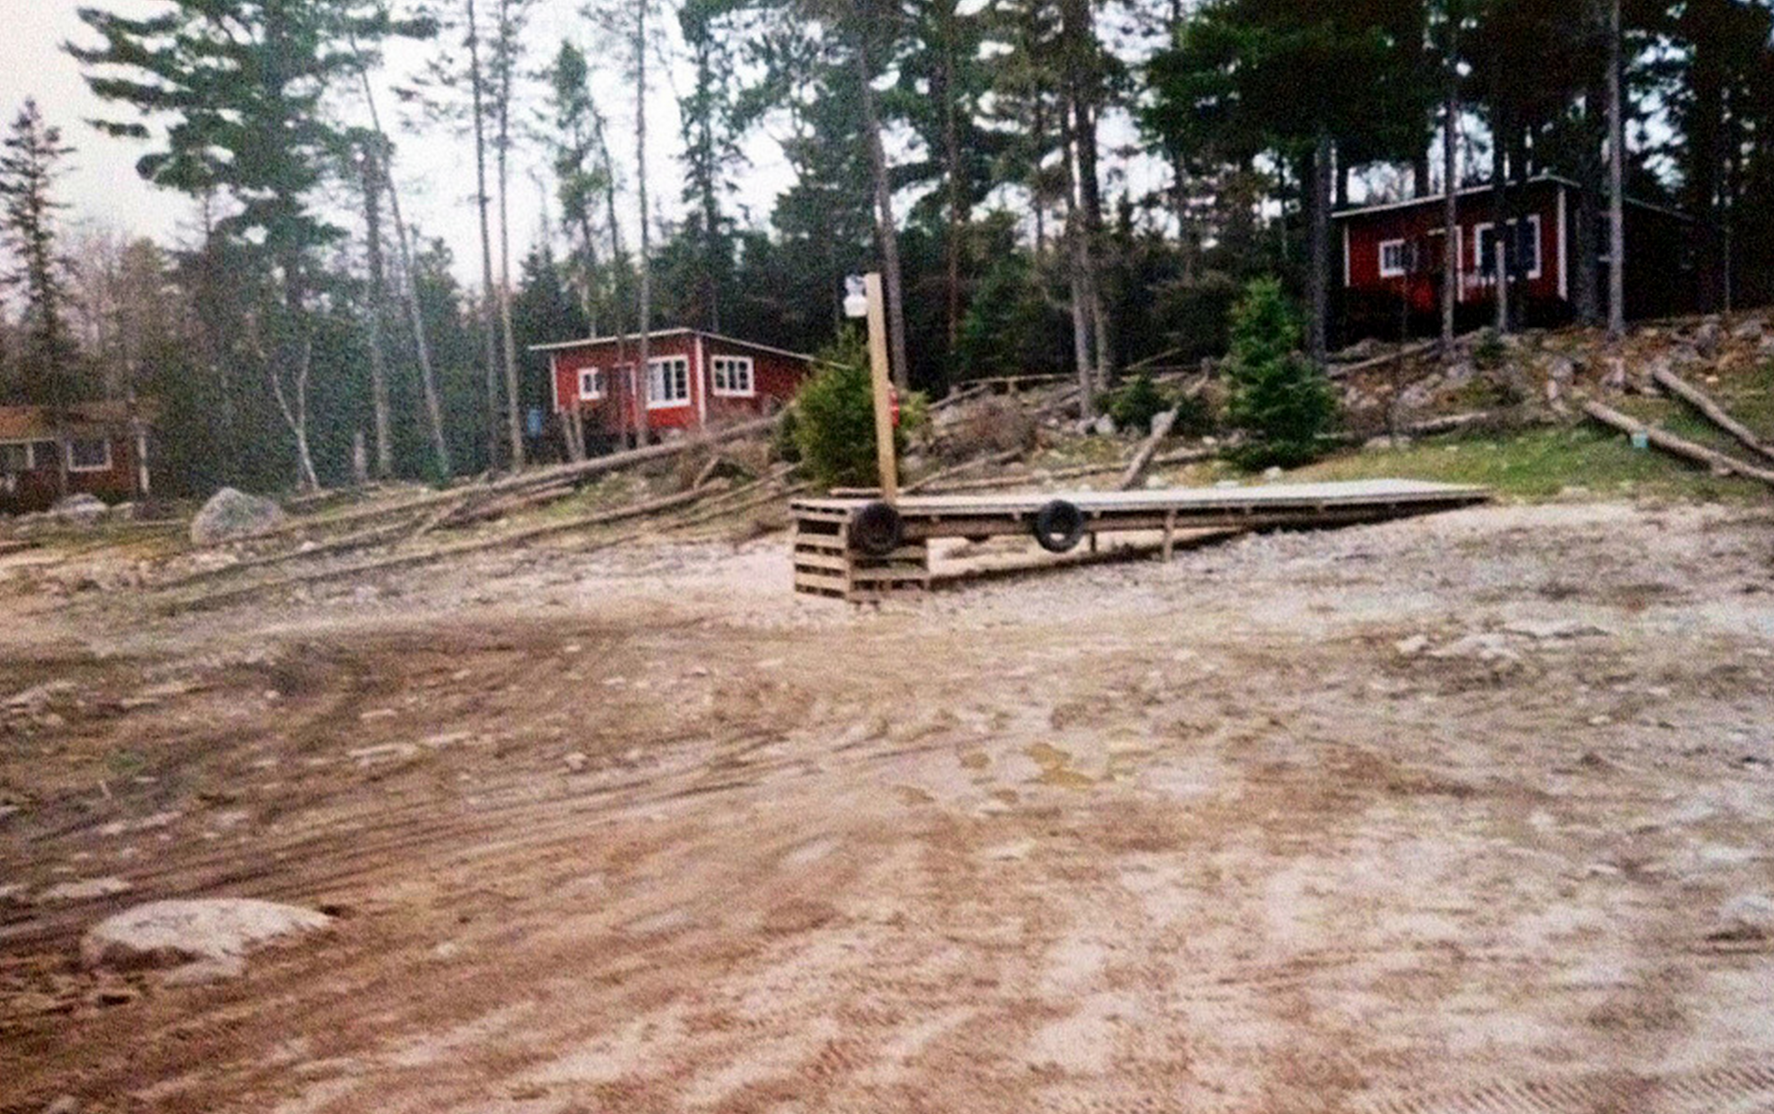
\includegraphics[height=\paperheight]{1987_drought_on_Kabetogama_2.png}}

\begin{frame}{1987 Low Water Year}

\footnotetext{\color{white}{Photo by Larry Kec}}

\end{frame}
}

%%%%%%%%%1%%%%%%%%%2%%%%%%%%%3%%%%%%%%%4%%%%%%%%%5%%%%%%%%%6%%%%%%%%%7%%%%%%%%%8

{{\usebackgroundtemplate%
	{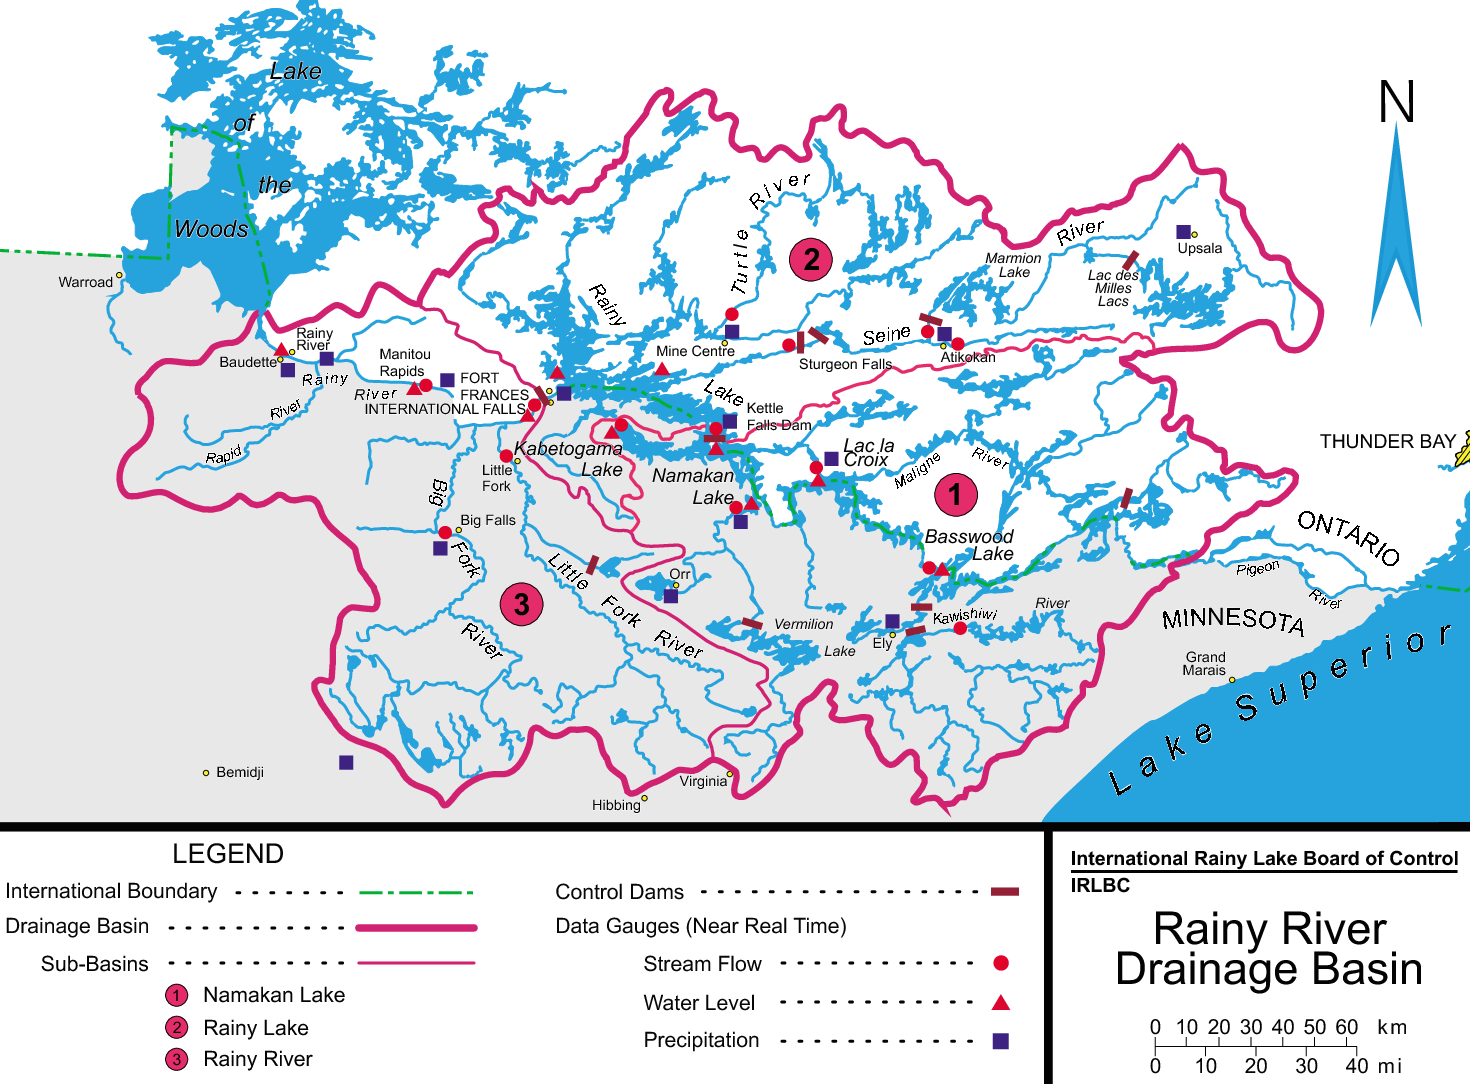
\includegraphics[width=\paperwidth]{75242923.png}}

\begin{frame}{}

\end{frame}
}

%%%%%%%%%1%%%%%%%%%2%%%%%%%%%3%%%%%%%%%4%%%%%%%%%5%%%%%%%%%6%%%%%%%%%7%%%%%%%%%8
\begin{frame}{Rainy River Mean Annual Flow}

\begin{center}
\includegraphicscopyright[width=0.8\paperwidth]{RainyRiverMeanAnnualFlowMAF.png}{Source: \href{http://jckantor.github.io/Rainy-Lake-Hydrology/}{Github Repository for this paper.}}
\end{center}

\hfill\begin{tabular}{lc}
& Million Acre-Feet/year \\
Rainy River at Fort Frances & 7.1 \\
Mississippi at St. Anthony Falls & 8.7 \\
Lake Mead Release at Hoover Dam & 9.6  \\
California, All managed Water & 40 \\
\end{tabular}\hfill
\end{frame}

%%%%%%%%%1%%%%%%%%%2%%%%%%%%%3%%%%%%%%%4%%%%%%%%%5%%%%%%%%%6%%%%%%%%%7%%%%%%%%%8
% Section 
%%%%%%%%%1%%%%%%%%%2%%%%%%%%%3%%%%%%%%%4%%%%%%%%%5%%%%%%%%%6%%%%%%%%%7%%%%%%%%%8

{\usebackgroundtemplate%
	{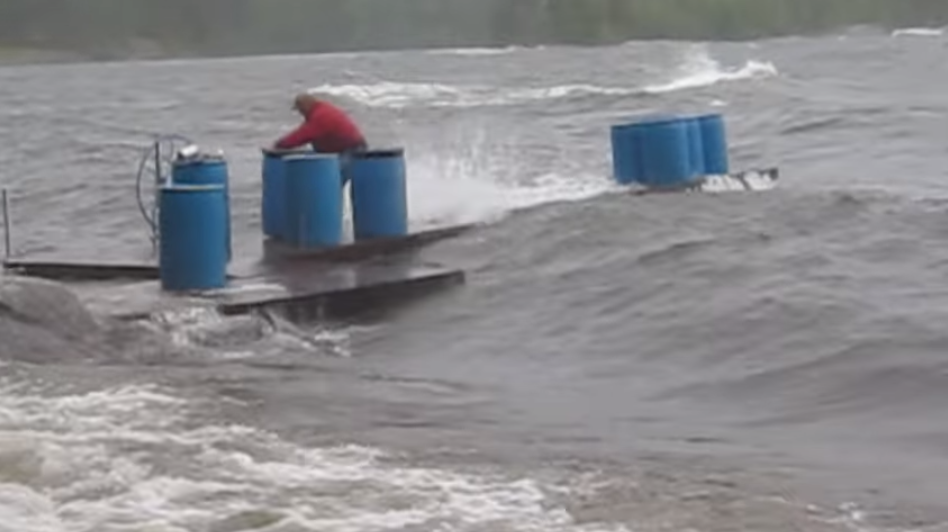
\includegraphics[height=\paperheight]{WaterBarrelsDock}}
\setbeamertemplate{footline}[text line]{some text}
\section{Impacts of the Rule Curve Change in 2000}
}

%%%%%%%%%1%%%%%%%%%2%%%%%%%%%3%%%%%%%%%4%%%%%%%%%5%%%%%%%%%6%%%%%%%%%7%%%%%%%%%8
\begin{frame}{International Joint Commission (IJC)}

Established by the Boundary Waters Treaty of 1909, the IJC is an "independent and objective advisor" to both countries regarding
 transboundary waters between the U.S. and Canada.
\begin{center}
\includegraphicscopyright[width=0.8\paperwidth]{IJC.jpg}{Source: \href{https://vertigo.revues.org/1885}{Vertigo Revues}}
\end{center}

\end{frame}


%%%%%%%%%1%%%%%%%%%2%%%%%%%%%3%%%%%%%%%4%%%%%%%%%5%%%%%%%%%6%%%%%%%%%7%%%%%%%%%8
\begin{frame}{Water Flow Namakan Reservoir through Rainy Lake}

\begin{center}
\includegraphicscopyright[width=0.8\paperwidth]{VOYA_Web_WaterFlowMap.jpg}{Source: US National Park Service}
\end{center}

\end{frame}

%%%%%%%%%1%%%%%%%%%2%%%%%%%%%3%%%%%%%%%4%%%%%%%%%5%%%%%%%%%6%%%%%%%%%7%%%%%%%%%8
\begin{frame}{Rainy Lake and Namakan Lake Levels 1911--}

Clearly see three rule curve regimes ...
\begin{center}
\includegraphicscopyright[width=0.75\paperwidth]{RainyNamakanLakeLevels.png}{Source: \href{http://jckantor.github.io/Rainy-Lake-Hydrology/}{Github Repository for this paper.}}
\end{center}

\end{frame}

%%%%%%%%%1%%%%%%%%%2%%%%%%%%%3%%%%%%%%%4%%%%%%%%%5%%%%%%%%%6%%%%%%%%%7%%%%%%%%%8
\begin{frame}{Rule Curve Performance 1970--1999}

\begin{center}
\includegraphicscopyright[width=0.8\paperwidth]{RuleCurvePerformance1970-1999.png}{Source: \href{http://jckantor.github.io/Rainy-Lake-Hydrology/}{Github Repository for this paper.}}
\end{center}

\end{frame}

%%%%%%%%%1%%%%%%%%%2%%%%%%%%%3%%%%%%%%%4%%%%%%%%%5%%%%%%%%%6%%%%%%%%%7%%%%%%%%%8
\begin{frame}{Rule Curve Performance 2000--2010}

\begin{center}
\includegraphicscopyright[width=0.8\paperwidth]{RuleCurvePerformance2000-2010.png}{Source: \href{http://jckantor.github.io/Rainy-Lake-Hydrology/}{Github Repository for this paper.}}
\end{center}

\end{frame}

%%%%%%%%%1%%%%%%%%%2%%%%%%%%%3%%%%%%%%%4%%%%%%%%%5%%%%%%%%%6%%%%%%%%%7%%%%%%%%%8
\begin{frame}{Summer High Water Events (May--September)}
\vfill
\hfill\begin{tabular}{lrrr}\toprule
\qquad\qquad\qquad\quad & & 1971--1999 & 2000--2010	\\
& & \unit[4437]{days} & \unit[1683]{days} \\
\midrule
\multicolumn{2}{l}{Rule Curve Exceeded} & & \\
& Frequency & 14.8\% & 17.8\% \\
& Median & \unit[0.07]{m} & \unit[0.23]{m}\\
& 95th Percentile & \unit[0.38]{m} & \unit[0.70]{m}\\
\midrule
\multicolumn{2}{l}{Emergency High Water} & & \\
& Frequency & 7.6\% & 13.7\%\\
& Median & \unit[0.05]{m} & \unit[0.19]{m} \\
& 95th Percentile & \unit[0.36]{m} & \unit[0.71]{m} \\
\midrule
\multicolumn{2}{l}{All Gates Open} & &\\
& Frequency & 1.9\% & 8.7\% \\
& Median & \unit[0.12]{m} & \unit[0.17]{m}\\
& 95th Percentile & \unit[0.29]{m} & \unit[0.62]{m} \\
\midrule
\end{tabular}\hfill

\vspace*{3mm}
\usebeamerfont{copyright text}{\usebeamercolor[fg]{copyright text}{Source: \href{http://jckantor.github.io/Rainy-Lake-Hydrology/}{Github Repository for this paper.}}}
\vfill

\end{frame}

%%%%%%%%%1%%%%%%%%%2%%%%%%%%%3%%%%%%%%%4%%%%%%%%%5%%%%%%%%%6%%%%%%%%%7%%%%%%%%%8
\begin{frame}{Rule Curve Changes in 2000}

\begin{center}
\includegraphicscopyright[width=0.8\paperwidth]{RuleCurveComparison.png}{Source: \href{http://jckantor.github.io/Rainy-Lake-Hydrology/}{Github Repository for this paper.}}
\end{center}

\end{frame}

%%%%%%%%%1%%%%%%%%%2%%%%%%%%%3%%%%%%%%%4%%%%%%%%%5%%%%%%%%%6%%%%%%%%%7%%%%%%%%%8
\begin{frame}{Imputed Change in Flows to Rainy River}

The change in rule curves implies a change in flows to Rainy River. Assuming midpoints of the rule curves ...
\begin{center}
\includegraphicscopyright[width=0.8\paperwidth]{ImputedChangeInFlows.png}{Source: \href{http://jckantor.github.io/Rainy-Lake-Hydrology/}{Github Repository for this paper.}}
\end{center}

\end{frame}

%%%%%%%%%1%%%%%%%%%2%%%%%%%%%3%%%%%%%%%4%%%%%%%%%5%%%%%%%%%6%%%%%%%%%7%%%%%%%%%8
\begin{frame}{Rainy Lake Inflows}

\centering

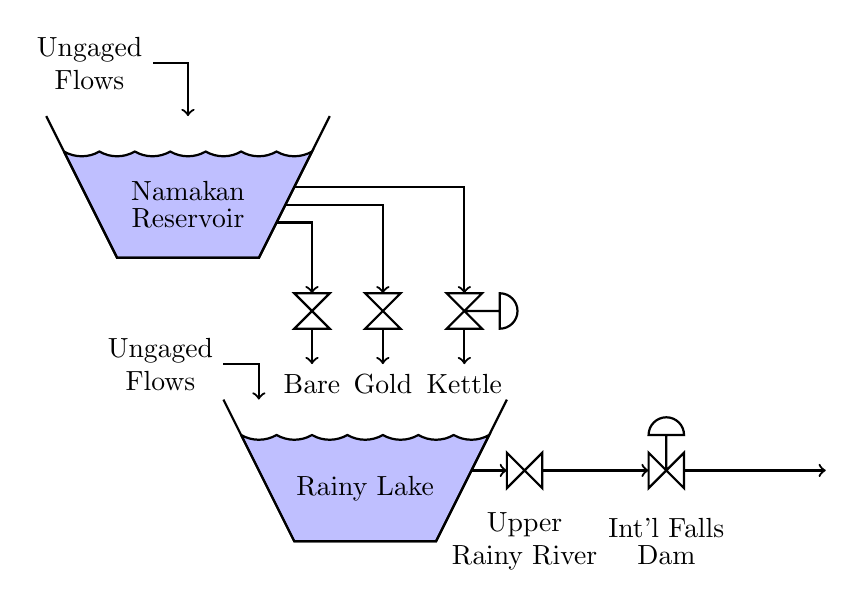
\begin{tikzpicture}[scale=0.9,thick]
\begin{sansmath}
  %\draw[step=1cm,gray,very thin] (0,0) grid (12,8);
  
  % Coordinates
  \coordinate (RL) at (3.5,2.5);
  \coordinate (NL) at (1,6.5); 
  \coordinate (Ranier) at (7.5,1.5);
  \coordinate (IFD) at (9.5,1.5);
  \coordinate (FT) at (11,1.5);
  \coordinate (Kettle) at (6.9,4);
  \coordinate (Gold) at (5.75,4);
  \coordinate (Bare) at (4.75,4);
  \coordinate (eqns) at (10,5.5);
  
  % Valve Symbols 
  \draw (IFD)--++(0,0.25)--++(0.5,-0.5)--++(0,0.5)--++(-0.5,-0.5)--++(0,0.25)
    ++(0.25,0)--++(0,0.5)--++(0.25,0) arc(0:180:0.25) --++(0.25,0);
  \draw (IFD)++(0.25,-1) node {\shortstack{Int'l Falls \\ Dam}};
  
  \draw (Ranier)--++(0,0.25)--++(0.5,-0.5)--++(0,0.5)--++(-0.5,-0.5)--++(0,0.25);
  \draw (Ranier)++(0.25,-1) node {\shortstack{Upper\\ Rainy River}};
  
  \draw (Kettle)--++(0.25,0)--++(-0.5,-0.5)--++(0.5,0)--++(-0.5,0.5)--++(0.25,0)
    ++(0,-0.25)--++(0.5,0)--++(0,-0.25) arc(-90:90:0.25cm)--++(0,-0.25);
  
  \draw (Gold)--++(0.25,0)--++(-0.5,-0.5)--++(0.5,0)--++(-0.5,0.5)--++(0.25,0);
  \draw (Bare)--++(0.25,0)--++(-0.5,-0.5)--++(0.5,0)--++(-0.5,0.5)--++(0.25,0);
  
  % Connectors
  \draw[<-] (Kettle)++(0,-1) node[below] {Kettle} --++(0,0.5);
  \draw[<-] (Kettle)--++(0,1.5)--++(-3,0);
  
  \draw[<-] (Gold)++(0,-1) node[below] {Gold} --++(0,0.5);
  \draw[<-] (Gold)--++(0,1.25)--++(-3,0);
  
  \draw[<-] (Bare)++(0,-1) node[below] {Bare} --++(0,0.5);
  \draw[<-] (Bare)--++(0,1.0)--++(-3,0);
  
  \draw[<-] (RL)++(0.5,0)--++(0,0.5)--++(-0.5,0) 
    node[left] {\shortstack{Ungaged \\ Flows}};
  \draw[<-] (NL)++(2,0)--++(0,0.75)--++(-0.5,0)
    node[left] {\shortstack{Ungaged \\ Flows}};
    
  \draw[<-] (Ranier)--++(-2,0);
  \draw[<-] (IFD)--++(-1.5,0);
  \draw[->] (IFD)++(0.5,0)--++(2,0);

  % Rainy Lake
  \draw[fill=blue!25] (RL) ++(0.25,-0.5)--++(0.75,-1.5)--++(2,0)--++(0.75,1.5)
    arc(-60:-120:0.5cm) arc(-60:-120:0.5cm) arc(-60:-120:0.5cm) arc(-60:-120:0.5cm)
    arc(-60:-120:0.5cm) arc(-60:-120:0.5cm) arc(-60:-120:0.5cm);
  \draw (RL)--++(1,-2)--++(2,0)--++(1,2);
  \draw (RL) ++(2,-1.25) node {\shortstack{Rainy Lake}};

  % Namakan Lake
  \draw[fill=blue!25] (NL) ++(0.25,-0.5)--++(0.75,-1.5)--++(2,0)--++(0.75,1.5)
    arc(-60:-120:0.5cm) arc(-60:-120:0.5cm) arc(-60:-120:0.5cm) arc(-60:-120:0.5cm)
    arc(-60:-120:0.5cm) arc(-60:-120:0.5cm) arc(-60:-120:0.5cm);
  \draw (NL)--++(1,-2)--++(2,0)--++(1,2);
  \draw (NL) ++(2,-1.25) node {\shortstack{Namakan \\ Reservoir}};
    
\end{sansmath}
\end{tikzpicture}

\end{frame}

%%%%%%%%%1%%%%%%%%%2%%%%%%%%%3%%%%%%%%%4%%%%%%%%%5%%%%%%%%%6%%%%%%%%%7%%%%%%%%%8
\begin{frame}{Rainy Lake Inflows, 1970-1999 vs 2000-2010}

\begin{center}
\includegraphicscopyright[width=0.8\paperwidth]{RainyLakeInflows.png}{Source: \href{http://jckantor.github.io/Rainy-Lake-Hydrology/}{Github Repository for this paper.}}
\end{center}

\end{frame}

%%%%%%%%%1%%%%%%%%%2%%%%%%%%%3%%%%%%%%%4%%%%%%%%%5%%%%%%%%%6%%%%%%%%%7%%%%%%%%%8
\begin{frame}{Change in Inflow to Rainy Lake, 1979-99 vs 2000-10}

\begin{center}
\includegraphicscopyright[width=0.8\paperwidth]{ChangeInMeanInflow.png}{Source: \href{http://jckantor.github.io/Rainy-Lake-Hydrology/}{Github Repository for this paper.}}
\end{center}

\end{frame}

%%%%%%%%%1%%%%%%%%%2%%%%%%%%%3%%%%%%%%%4%%%%%%%%%5%%%%%%%%%6%%%%%%%%%7%%%%%%%%%8
% Section 
%%%%%%%%%1%%%%%%%%%2%%%%%%%%%3%%%%%%%%%4%%%%%%%%%5%%%%%%%%%6%%%%%%%%%7%%%%%%%%%8

{\usebackgroundtemplate%
	{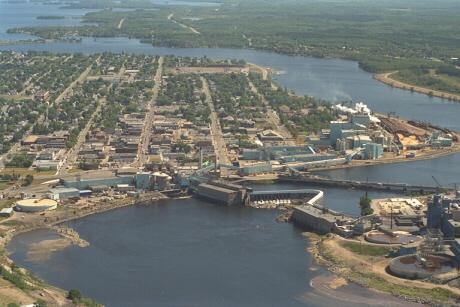
\includegraphics[height=\paperheight]{mill.jpg}}
\section{Bottleneck at Rainy River}
}
 
%%%%%%%%%1%%%%%%%%%2%%%%%%%%%3%%%%%%%%%4%%%%%%%%%5%%%%%%%%%6%%%%%%%%%7%%%%%%%%%8
\begin{frame}{Railroad Bridge at Ranier, 190x versus 2015}

\begin{center}
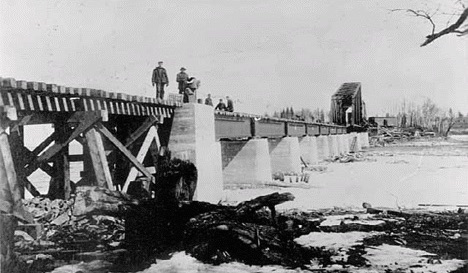
\includegraphics[height=0.4\paperheight]{RailBridgeRanier.jpg}
\end{center}
\vfil
\begin{center}
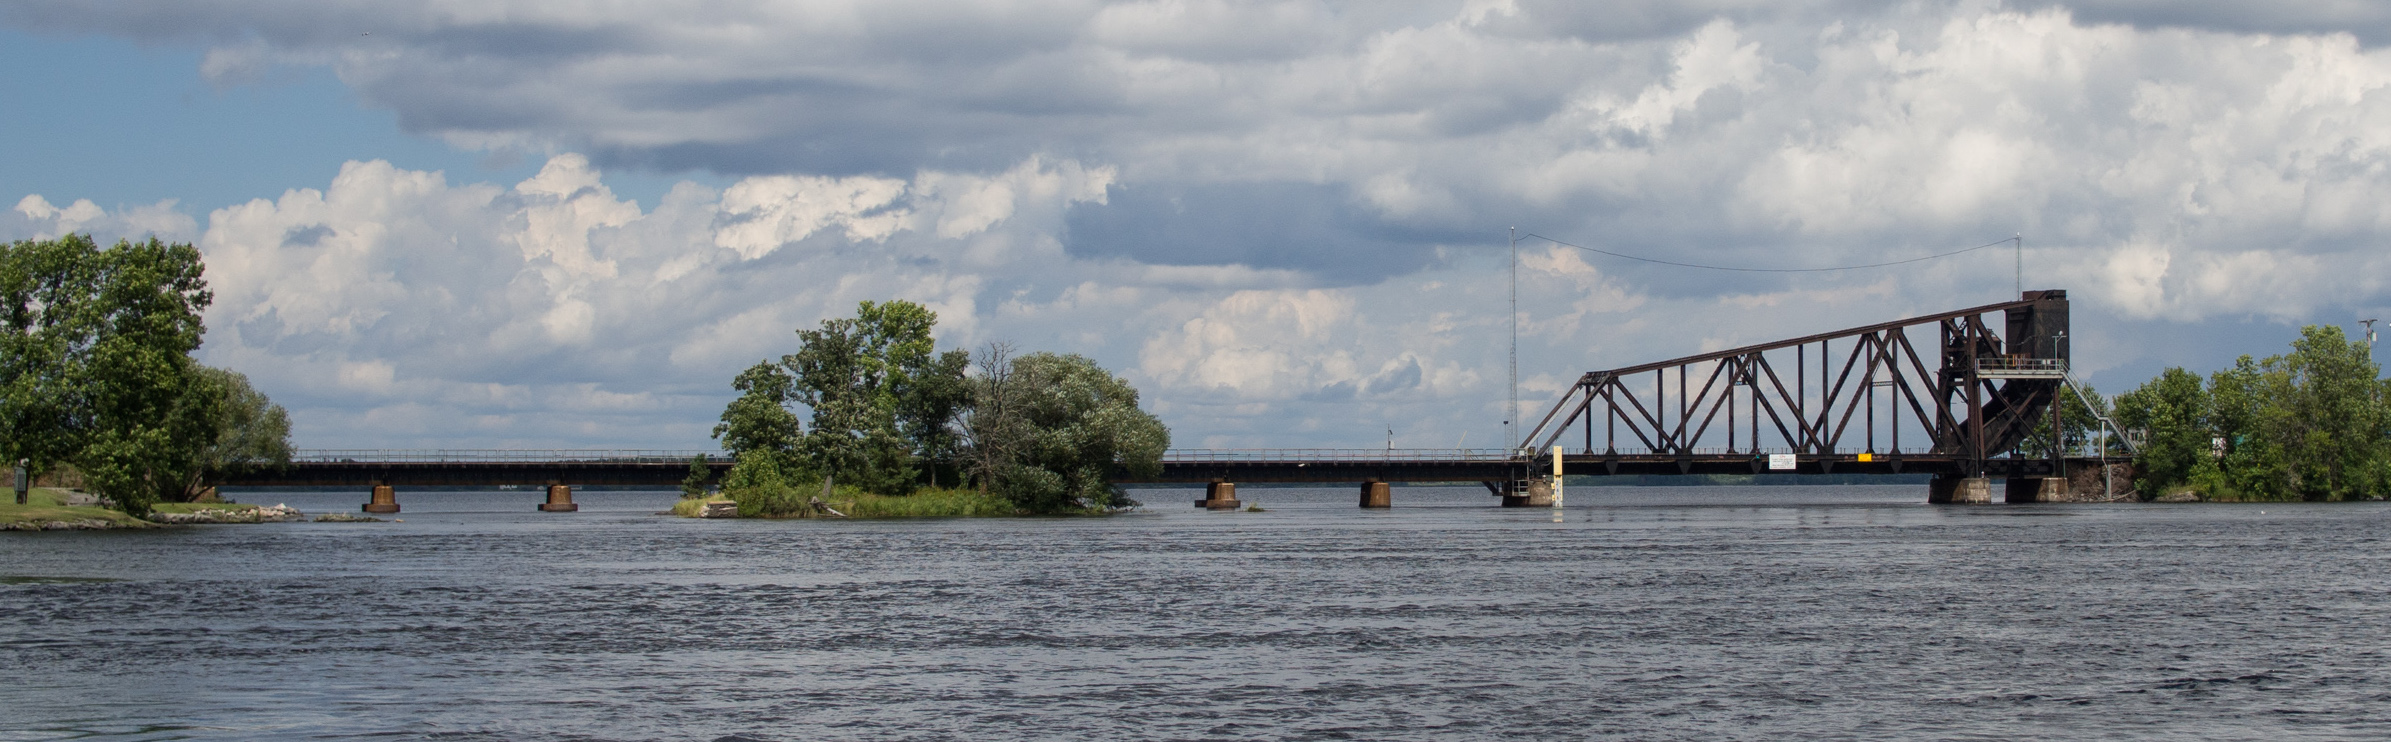
\includegraphics[height=0.32\paperheight]{20150808_142421.jpg}
\end{center}

\end{frame}

%%%%%%%%%1%%%%%%%%%2%%%%%%%%%3%%%%%%%%%4%%%%%%%%%5%%%%%%%%%6%%%%%%%%%7%%%%%%%%%8
\begin{frame}{Flow Constrictions on Upper Rainy River}

Constrictions at Ranier limit the discharge rate from Rainy Lake
\begin{center}
\includegraphicscopyright[height=0.7\paperheight]{RainyRiverConstrictions.png}{Source: \href{http://jckantor.github.io/Rainy-Lake-Hydrology/}{Github Repository for this paper.}}
\end{center}

\end{frame}

%%%%%%%%%1%%%%%%%%%2%%%%%%%%%3%%%%%%%%%4%%%%%%%%%5%%%%%%%%%6%%%%%%%%%7%%%%%%%%%8
\begin{frame}{Rainy River Discharge 1970--2010}

\begin{center}
\includegraphicscopyright[width=0.8\paperwidth]{RainyRiverDischarge.png}{Source: \href{http://jckantor.github.io/Rainy-Lake-Hydrology/}{Github Repository for this paper.}}
\end{center}

\end{frame}

%%%%%%%%%1%%%%%%%%%2%%%%%%%%%3%%%%%%%%%4%%%%%%%%%5%%%%%%%%%6%%%%%%%%%7%%%%%%%%%8
\begin{frame}{Impact of the Rule Curve Change, 1970 - 2000}

\begin{enumerate}
\item Displaces winter inflow to Rainy Lake from winter to summer months.
\item Flow constrictions in Upper Rainy River lead to water level increases in May/June.
\end{enumerate}

\end{frame}

%%%%%%%%%1%%%%%%%%%2%%%%%%%%%3%%%%%%%%%4%%%%%%%%%5%%%%%%%%%6%%%%%%%%%7%%%%%%%%%8
% Section 
%%%%%%%%%1%%%%%%%%%2%%%%%%%%%3%%%%%%%%%4%%%%%%%%%5%%%%%%%%%6%%%%%%%%%7%%%%%%%%%8

{\usebackgroundtemplate%
	{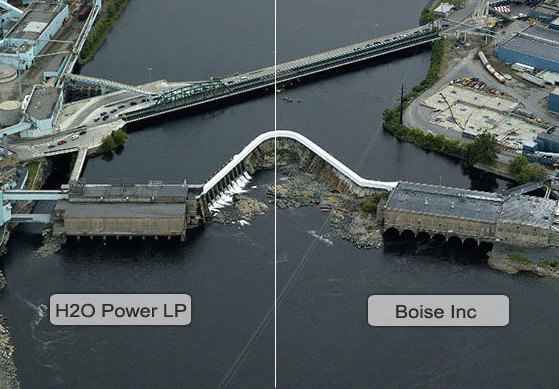
\includegraphics[height=\paperheight]{fort-frances-split.jpg}}
\section{Improving Control of Lake Levels}
}

%%%%%%%%%1%%%%%%%%%2%%%%%%%%%3%%%%%%%%%4%%%%%%%%%5%%%%%%%%%6%%%%%%%%%7%%%%%%%%%8
\begin{frame}{Current Practice}

\centering

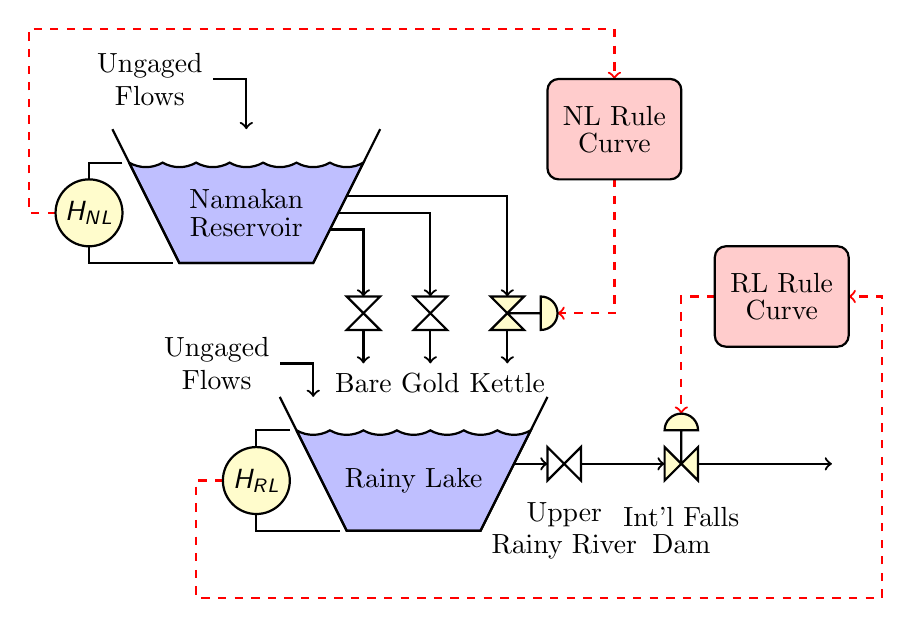
\begin{tikzpicture}[scale=0.85,thick]
\begin{sansmath}
  %\draw[step=1cm,gray,very thin] (0,0) grid (12,8);
  
  % Coordinates
  \coordinate (RL) at (3.5,2.5);
  \coordinate (NL) at (1,6.5); 
  \coordinate (Ranier) at (7.5,1.5);
  \coordinate (IFD) at (9.25,1.5);
  \coordinate (Kettle) at (6.9,4);
  \coordinate (Gold) at (5.75,4);
  \coordinate (Bare) at (4.75,4);
  \coordinate (control) at (11,4);
  \coordinate (control2) at (8.5,6.5);
  
  % Control lines
  \draw[dashed,->,color=red] (RL)++(-0.35,-1.25)--++(-0.9,0)--++(0,-1.75) 
    --++(10.25,0)--++(0,4.5)--++(-0.5,0);
  \draw[dashed,->,color=red] (control)--++(-1.5,0)--++(0,-1.75);
  \draw[dashed,->,color=red] (NL)++(-0.35,-1.25)--++(-0.9,0)--++(0,2.75)
    --++(8.75,0)--++(0,-0.75);
  \draw[dashed,->,color=red] (control2)--++(0,-2.75)--++(-0.85,0);
    
  % Valve Symbols 
  \draw[fill=yellow!20] (IFD)--++(0,0.25)--++(0.5,-0.5)--++(0,0.5)
    --++(-0.5,-0.5)--++(0,0.25)
    ++(0.25,0)--++(0,0.5)--++(0.25,0) arc(0:180:0.25) --++(0.25,0);
  \draw (IFD)++(0.25,-1) node {\shortstack{Int'l Falls \\ Dam}};
  
  \draw (Ranier)--++(0,0.25)--++(0.5,-0.5)--++(0,0.5)--++(-0.5,-0.5)--++(0,0.25);
  \draw (Ranier)++(0.25,-1) node {\shortstack{Upper\\ Rainy River}};
  
  \draw[fill=yellow!20] (Kettle)--++(0.25,0)--++(-0.5,-0.5)--++(0.5,0)--++(-0.5,0.5)--++(0.25,0)
    ++(0,-0.25)--++(0.5,0)--++(0,-0.25) arc(-90:90:0.25cm)--++(0,-0.25);
  
  \draw (Gold)--++(0.25,0)--++(-0.5,-0.5)--++(0.5,0)--++(-0.5,0.5)--++(0.25,0);
  \draw (Bare)--++(0.25,0)--++(-0.5,-0.5)--++(0.5,0)--++(-0.5,0.5)--++(0.25,0);
 
  % Level Transmitter
  \draw (RL) ++(0.15,-0.5)--++(-0.5,0)--++(0,-1.5) --++(1.25,0);
  \draw[fill=yellow!20] (RL) ++(-0.35,-0.75) arc(-270:90:0.5cm) 
    ++(0,-0.5) node {$H_{RL}$};
        
  \draw (NL) ++(0.15,-0.5)--++(-0.5,0)--++(0,-1.5) --++(1.25,0);
  \draw[fill=yellow!20] (NL) ++(-0.35,-0.75) arc(-270:90:0.5cm) 
    ++(0,-0.5) node {$H_{NL}$};
  
  % Connectors
  \draw[<-] (Kettle)++(0,-1.0) node[below] {Kettle} --++(0,0.5);
  \draw[<-] (Kettle)--++(0,1.5)--++(-3,0);
  
  \draw[<-] (Gold)++(0,-1) node[below] {Gold} --++(0,0.5);
  \draw[<-] (Gold)--++(0,1.25)--++(-3,0);
  
  \draw[<-] (Bare)++(0,-1) node[below] {Bare} --++(0,0.5);
  \draw[<-] (Bare)--++(0,1.0)--++(-3,0);
  
  \draw[<-] (RL)++(0.5,0)--++(0,0.5)--++(-0.5,0) 
    node[left] {\shortstack{Ungaged \\ Flows}};
  \draw[<-] (NL)++(2,0)--++(0,0.75)--++(-0.5,0)
    node[left] {\shortstack{Ungaged \\ Flows}};
    
  \draw[<-] (Ranier)--++(-2,0);
  \draw[<-] (IFD)--++(-1.25,0);
  \draw[->] (IFD)++(0.5,0)--++(2,0);
  
  % Rainy Lake
  \draw[fill=blue!25] (RL) ++(0.25,-0.5)--++(0.75,-1.5)--++(2,0)--++(0.75,1.5)
    arc(-60:-120:0.5cm) arc(-60:-120:0.5cm) arc(-60:-120:0.5cm) arc(-60:-120:0.5cm)
    arc(-60:-120:0.5cm) arc(-60:-120:0.5cm) arc(-60:-120:0.5cm);
  \draw (RL)--++(1,-2)--++(2,0)--++(1,2);
  \draw (RL) ++(2,-1.25) node {\shortstack{Rainy Lake}};

  % Namakan Lake
  \draw[fill=blue!25] (NL) ++(0.25,-0.5)--++(0.75,-1.5)--++(2,0)--++(0.75,1.5)
    arc(-60:-120:0.5cm) arc(-60:-120:0.5cm) arc(-60:-120:0.5cm) arc(-60:-120:0.5cm)
    arc(-60:-120:0.5cm) arc(-60:-120:0.5cm) arc(-60:-120:0.5cm);
  \draw (NL)--++(1,-2)--++(2,0)--++(1,2);
  \draw (NL) ++(2,-1.25) node {\shortstack{Namakan \\ Reservoir}};
  
  % Controller
  \draw[rounded corners,fill=red!20] (control) 
    +(-1,-0.75) rectangle +(1,0.75);
  \draw (control) node {\shortstack{RL Rule\\ Curve}};
    
  \draw[rounded corners,fill=red!20] (control2) 
    +(-1,-0.75) rectangle +(1,0.75);
  \draw (control2) node {\shortstack{NL Rule\\ Curve}};
      
\end{sansmath}
\end{tikzpicture}

\end{frame}

%%%%%%%%%1%%%%%%%%%2%%%%%%%%%3%%%%%%%%%4%%%%%%%%%5%%%%%%%%%6%%%%%%%%%7%%%%%%%%%8
\begin{frame}{Model Predictive Control for Rainy Lake}

\centering

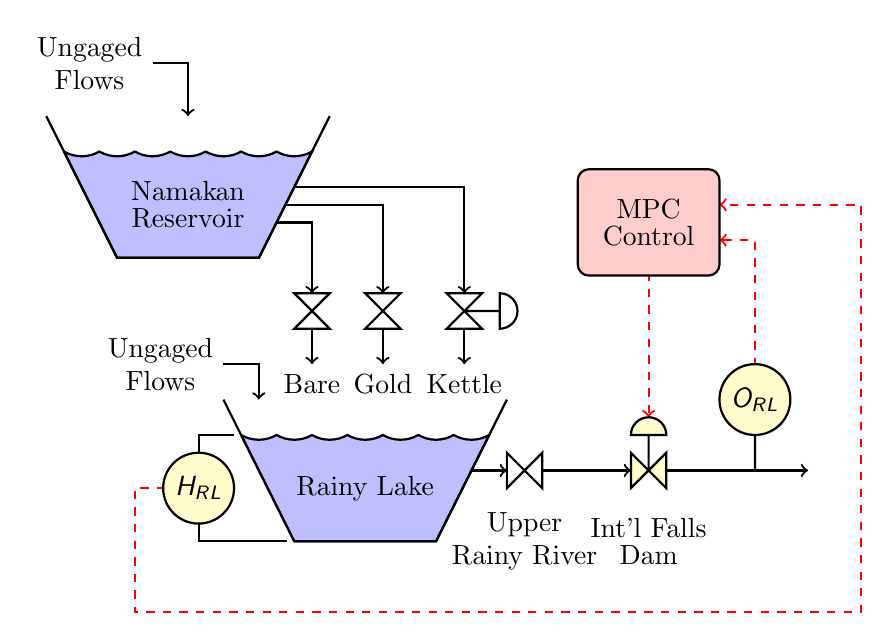
\begin{tikzpicture}[scale=0.9,thick]
\begin{sansmath}
  %\draw[step=1cm,gray,very thin] (0,0) grid (12,8);
  
  % Coordinates
  \coordinate (RL) at (3.5,2.5);
  \coordinate (NL) at (1,6.5); 
  \coordinate (Ranier) at (7.5,1.5);
  \coordinate (IFD) at (9.25,1.5);
  \coordinate (FT) at (11,1.5);
  \coordinate (Kettle) at (6.9,4);
  \coordinate (Gold) at (5.75,4);
  \coordinate (Bare) at (4.75,4);
  \coordinate (control) at (9.5,5);
  
  % Control lines
  \draw[dashed,->,color=red] (RL)++(-0.35,-1.25)--++(-0.9,0)--++(0,-1.75) 
    --++(10.25,0)--++(0,5.75)--++(-2,0);
  \draw[dashed,->,color=red] (FT)++(0,1)--++(0,2.25)--++(-0.5,0);
  \draw[dashed,->,color=red] (control)--++(0,-2.75);
  
  % Valve Symbols 
  \draw[fill=yellow!20] (IFD)--++(0,0.25)--++(0.5,-0.5)--++(0,0.5)
    --++(-0.5,-0.5)--++(0,0.25)
    ++(0.25,0)--++(0,0.5)--++(0.25,0) arc(0:180:0.25) --++(0.25,0);
  \draw (IFD)++(0.25,-1) node {\shortstack{Int'l Falls \\ Dam}};
  
  \draw (Ranier)--++(0,0.25)--++(0.5,-0.5)--++(0,0.5)--++(-0.5,-0.5)--++(0,0.25);
  \draw (Ranier)++(0.25,-1) node {\shortstack{Upper\\ Rainy River}};
  
  \draw (Kettle)--++(0.25,0)--++(-0.5,-0.5)--++(0.5,0)--++(-0.5,0.5)--++(0.25,0)
    ++(0,-0.25)--++(0.5,0)--++(0,-0.25) arc(-90:90:0.25cm)--++(0,-0.25);
  
  \draw (Gold)--++(0.25,0)--++(-0.5,-0.5)--++(0.5,0)--++(-0.5,0.5)--++(0.25,0);
  \draw (Bare)--++(0.25,0)--++(-0.5,-0.5)--++(0.5,0)--++(-0.5,0.5)--++(0.25,0);
  
  % Flow Transmitter
  \draw[fill=yellow!20] (FT)--++(0,0.5) arc(-90:270:0.5cm) ++(0,0.5) node {$O_{RL}$};
 
  % Level Transmitter
  \draw (RL) ++(0.15,-0.5)--++(-0.5,0)--++(0,-1.5) --++(1.25,0);
  \draw[fill=yellow!20] (RL) ++(-0.35,-0.75) arc(-270:90:0.5cm) 
    ++(0,-0.5) node {$H_{RL}$};
  
  % Connectors
  \draw[<-] (Kettle)++(0,-1.0) node[below] {Kettle} --++(0,0.5);
  \draw[<-] (Kettle)--++(0,1.5)--++(-3,0);
  
  \draw[<-] (Gold)++(0,-1) node[below] {Gold} --++(0,0.5);
  \draw[<-] (Gold)--++(0,1.25)--++(-3,0);
  
  \draw[<-] (Bare)++(0,-1) node[below] {Bare} --++(0,0.5);
  \draw[<-] (Bare)--++(0,1.0)--++(-3,0);
  
  \draw[<-] (RL)++(0.5,0)--++(0,0.5)--++(-0.5,0) 
    node[left] {\shortstack{Ungaged \\ Flows}};
  \draw[<-] (NL)++(2,0)--++(0,0.75)--++(-0.5,0)
    node[left] {\shortstack{Ungaged \\ Flows}};
    
  \draw[<-] (Ranier)--++(-2,0);
  \draw[<-] (IFD)--++(-1.25,0);
  \draw[->] (IFD)++(0.5,0)--++(2,0);
  
  % Rainy Lake
  \draw[fill=blue!25] (RL) ++(0.25,-0.5)--++(0.75,-1.5)--++(2,0)--++(0.75,1.5)
    arc(-60:-120:0.5cm) arc(-60:-120:0.5cm) arc(-60:-120:0.5cm) arc(-60:-120:0.5cm)
    arc(-60:-120:0.5cm) arc(-60:-120:0.5cm) arc(-60:-120:0.5cm);
  \draw (RL)--++(1,-2)--++(2,0)--++(1,2);
  \draw (RL) ++(2,-1.25) node {\shortstack{Rainy Lake}};

  % Namakan Lake
  \draw[fill=blue!25] (NL) ++(0.25,-0.5)--++(0.75,-1.5)--++(2,0)--++(0.75,1.5)
    arc(-60:-120:0.5cm) arc(-60:-120:0.5cm) arc(-60:-120:0.5cm) arc(-60:-120:0.5cm)
    arc(-60:-120:0.5cm) arc(-60:-120:0.5cm) arc(-60:-120:0.5cm);
  \draw (NL)--++(1,-2)--++(2,0)--++(1,2);
  \draw (NL) ++(2,-1.25) node {\shortstack{Namakan \\ Reservoir}};
  
  % Controller
    \draw[rounded corners,fill=red!20] (control) 
      +(-1,-0.75) rectangle +(1,0.75);
    \draw (control) node {\shortstack{MPC\\ Control}};
      
\end{sansmath}
\end{tikzpicture}

\end{frame}
 
%%%%%%%%%1%%%%%%%%%2%%%%%%%%%3%%%%%%%%%4%%%%%%%%%5%%%%%%%%%6%%%%%%%%%7%%%%%%%%%8
\begin{frame}{Matlab/Simulink Simulation}

A calibrated Matlab/Simulink model of single loop control and full implemention of the 2000 IJC Order for Rainy Lake.

\vfill
\centering
\includegraphicscopyright[width=0.85\paperwidth]{Rainy_Lake_Simulation_Model}{Source: \href{http://jckantor.github.io/Rainy-Lake-Hydrology/}{Github Repository for this paper.}}
\vfill

\end{frame}
 
%%%%%%%%%1%%%%%%%%%2%%%%%%%%%3%%%%%%%%%4%%%%%%%%%5%%%%%%%%%6%%%%%%%%%7%%%%%%%%%8
\begin{frame}{Simulation Results for Rainy Lake}
\vfill
\centering
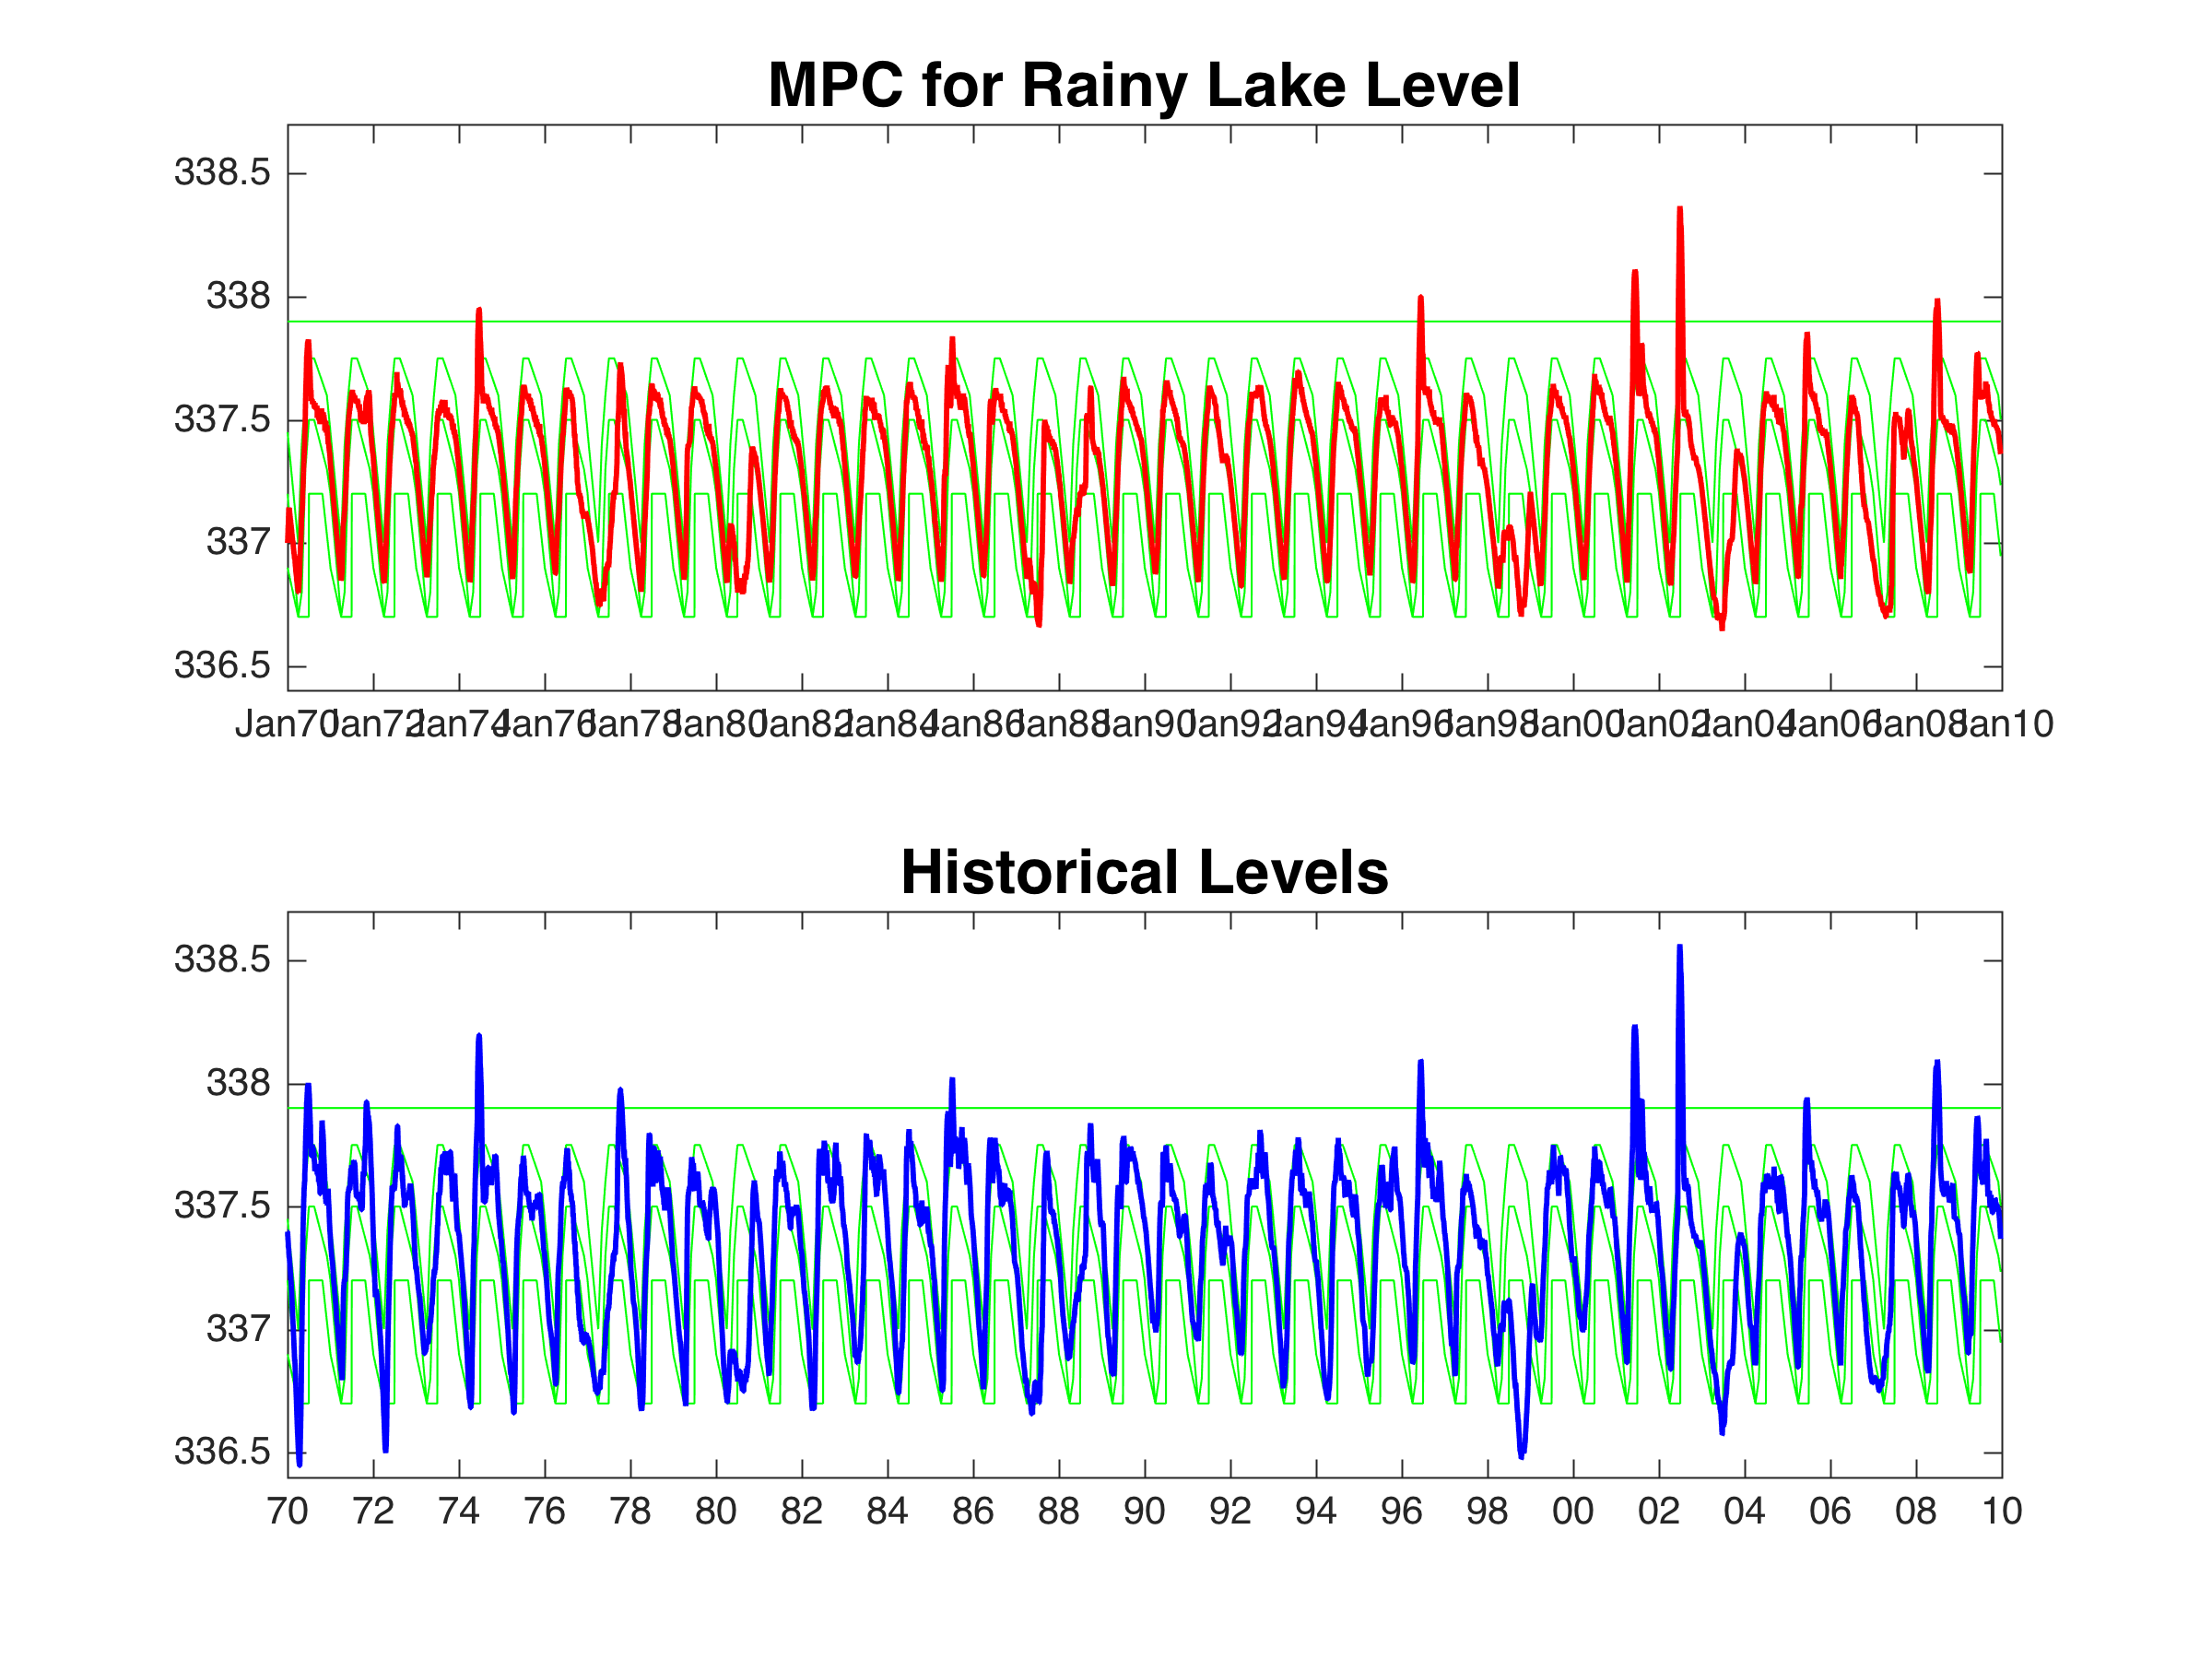
\includegraphics[height=0.85\paperheight]{Rainy_Lake_Simulation_Results}
\vfill
 
\end{frame}
 
%%%%%%%%%1%%%%%%%%%2%%%%%%%%%3%%%%%%%%%4%%%%%%%%%5%%%%%%%%%6%%%%%%%%%7%%%%%%%%%8
\begin{frame}{Integrated Control of Namakan and Rainy Lake}

\centering

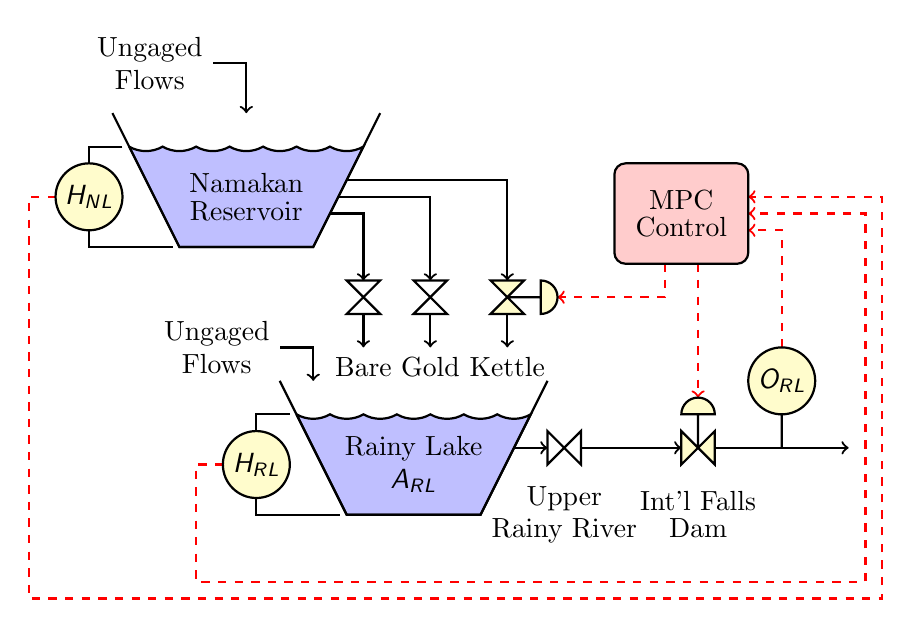
\begin{tikzpicture}[scale=0.85,thick]
\begin{sansmath}
  %\draw[step=1cm,gray,very thin] (0,0) grid (12,8);
  
  % Coordinates
  \coordinate (RL) at (3.5,2.5);
  \coordinate (NL) at (1,6.5); 
  \coordinate (Ranier) at (7.5,1.5);
  \coordinate (IFD) at (9.5,1.5);
  \coordinate (FT) at (11,1.5);
  \coordinate (Kettle) at (6.9,4);
  \coordinate (Gold) at (5.75,4);
  \coordinate (Bare) at (4.75,4);
  \coordinate (control) at (9.5,5);
  
  % Control lines
  \draw[dashed,->,color=red] (RL)++(-0.35,-1.25)--++(-0.9,0)--++(0,-1.75) 
    --++(10,0)--++(0,5.5)--++(-1.75,0);
  \draw[dashed,->,color=red] (NL)++(-0.35,-1.25)--++(-0.9,0)--++(0,-6) 
    --++(12.75,0)--++(0,6)--++(-2,0);
  \draw[dashed,->,color=red] (FT)++(0,1)--++(0,2.25)--++(-0.5,0);
  \draw[dashed,->,color=red] (control)++(0.25,0)--++(0,-2.75);
  \draw[dashed,->,color=red] (control)++(-0.25,0)--++(0,-1.25)--++(-1.6,0);
  
  % Valve Symbols 
  \draw[fill=yellow!20] (IFD)--++(0,0.25)--++(0.5,-0.5)--++(0,0.5)
    --++(-0.5,-0.5)--++(0,0.25)
    ++(0.25,0)--++(0,0.5)--++(0.25,0) arc(0:180:0.25) --++(0.25,0);
  \draw (IFD)++(0.25,-1) node {\shortstack{Int'l Falls \\ Dam}};
  
  \draw (Ranier)--++(0,0.25)--++(0.5,-0.5)--++(0,0.5)--++(-0.5,-0.5)--++(0,0.25);
  \draw (Ranier)++(0.25,-1) node {\shortstack{Upper\\ Rainy River}};
  
  \draw[fill=yellow!20] (Kettle)--++(0.25,0)--++(-0.5,-0.5)--++(0.5,0)--++(-0.5,0.5)--++(0.25,0)
    ++(0,-0.25)--++(0.5,0)--++(0,-0.25) arc(-90:90:0.25cm)--++(0,-0.25);
  
  \draw (Gold)--++(0.25,0)--++(-0.5,-0.5)--++(0.5,0)--++(-0.5,0.5)--++(0.25,0);
  \draw (Bare)--++(0.25,0)--++(-0.5,-0.5)--++(0.5,0)--++(-0.5,0.5)--++(0.25,0);
  
  % Flow Transmitter
  \draw[fill=yellow!20] (FT)--++(0,0.5) arc(-90:270:0.5cm) ++(0,0.5) node {$O_{RL}$};
 
  % Level Transmitter
  \draw (RL) ++(0.15,-0.5)--++(-0.5,0)--++(0,-1.5) --++(1.25,0);
  \draw[fill=yellow!20] (RL) ++(-0.35,-0.75) arc(-270:90:0.5cm) 
    ++(0,-0.5) node {$H_{RL}$};
    
  \draw (NL) ++(0.15,-0.5)--++(-0.5,0)--++(0,-1.5) --++(1.25,0);
  \draw[fill=yellow!20] (NL) ++(-0.35,-0.75) arc(-270:90:0.5cm) 
    ++(0,-0.5) node {$H_{NL}$};
  
  % Connectors
  \draw[<-] (Kettle)++(0,-1.0) node[below] {Kettle} --++(0,0.5);
  \draw[<-] (Kettle)--++(0,1.5)--++(-3,0);
  
  \draw[<-] (Gold)++(0,-1) node[below] {Gold} --++(0,0.5);
  \draw[<-] (Gold)--++(0,1.25)--++(-3,0);
  
  \draw[<-] (Bare)++(0,-1) node[below] {Bare} --++(0,0.5);
  \draw[<-] (Bare)--++(0,1.0)--++(-3,0);
  
  \draw[<-] (RL)++(0.5,0)--++(0,0.5)--++(-0.5,0) 
    node[left] {\shortstack{Ungaged \\ Flows}};
  \draw[<-] (NL)++(2,0)--++(0,0.75)--++(-0.5,0)
    node[left] {\shortstack{Ungaged \\ Flows}};
    
  \draw[<-] (Ranier)--++(-2,0);
  \draw[<-] (IFD)--++(-1.5,0);
  \draw[->] (IFD)++(0.5,0)--++(2,0);
  
  % Rainy Lake
  \draw[fill=blue!25] (RL) ++(0.25,-0.5)--++(0.75,-1.5)--++(2,0)--++(0.75,1.5)
    arc(-60:-120:0.5cm) arc(-60:-120:0.5cm) arc(-60:-120:0.5cm) arc(-60:-120:0.5cm)
    arc(-60:-120:0.5cm) arc(-60:-120:0.5cm) arc(-60:-120:0.5cm);
  \draw (RL)--++(1,-2)--++(2,0)--++(1,2);
  \draw (RL) ++(2,-1.25) node {\shortstack{Rainy Lake \\ $A_{RL}$}};

  % Namakan Lake
  \draw[fill=blue!25] (NL) ++(0.25,-0.5)--++(0.75,-1.5)--++(2,0)--++(0.75,1.5)
    arc(-60:-120:0.5cm) arc(-60:-120:0.5cm) arc(-60:-120:0.5cm) arc(-60:-120:0.5cm)
    arc(-60:-120:0.5cm) arc(-60:-120:0.5cm) arc(-60:-120:0.5cm);
  \draw (NL)--++(1,-2)--++(2,0)--++(1,2);
  \draw (NL) ++(2,-1.25) node {\shortstack{Namakan \\ Reservoir}};
  
  % Controller
    \draw[rounded corners,fill=red!20] (control) 
      +(-1,-0.75) rectangle +(1,0.75);
    \draw (control) node {\shortstack{MPC\\ Control}};
      
\end{sansmath}
\end{tikzpicture}

\end{frame}

%%%%%%%%%1%%%%%%%%%2%%%%%%%%%3%%%%%%%%%4%%%%%%%%%5%%%%%%%%%6%%%%%%%%%7%%%%%%%%%8
\begin{frame}{Rainy Lake Levels 2015}
\vfill
\centering
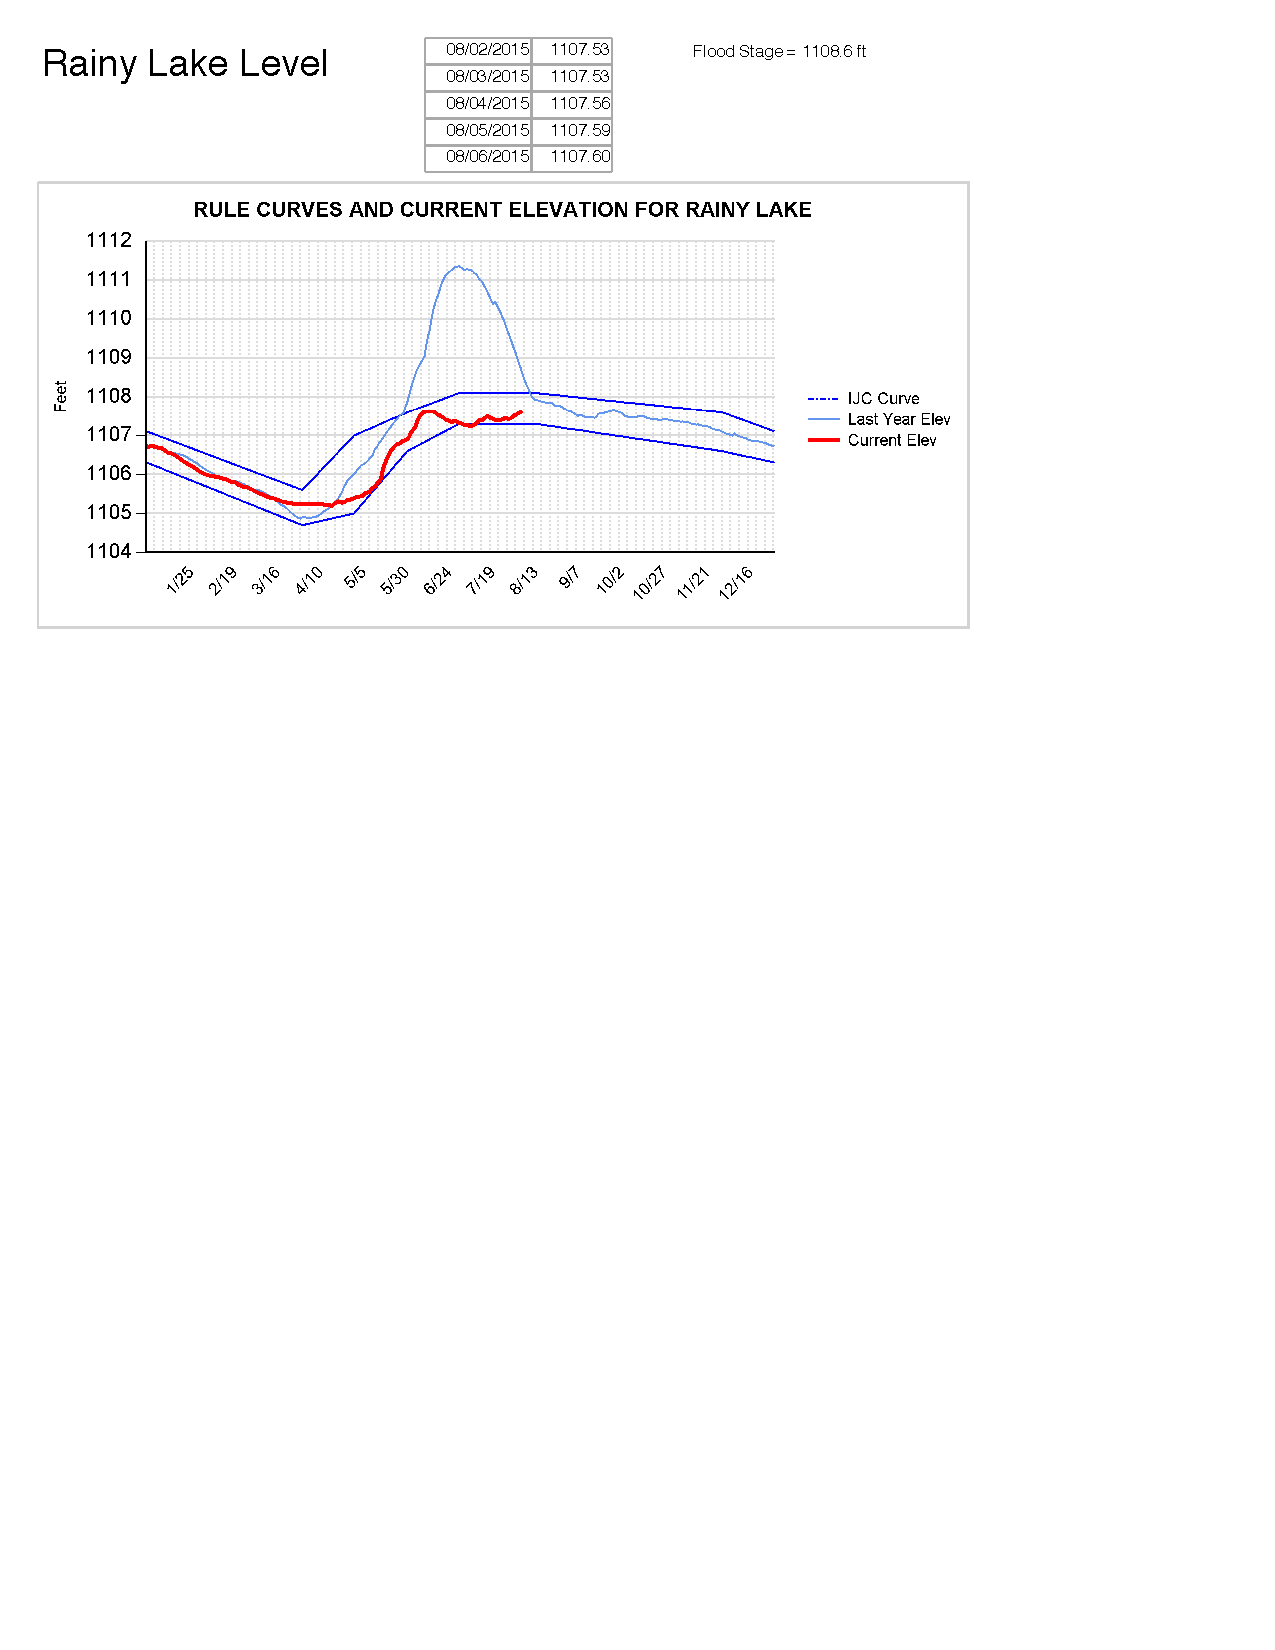
\includegraphics[width=0.85\paperwidth]{RainyLevel}
\vfill
 
\end{frame}

%%%%%%%%%1%%%%%%%%%2%%%%%%%%%3%%%%%%%%%4%%%%%%%%%5%%%%%%%%%6%%%%%%%%%7%%%%%%%%%8

{{\usebackgroundtemplate%
	{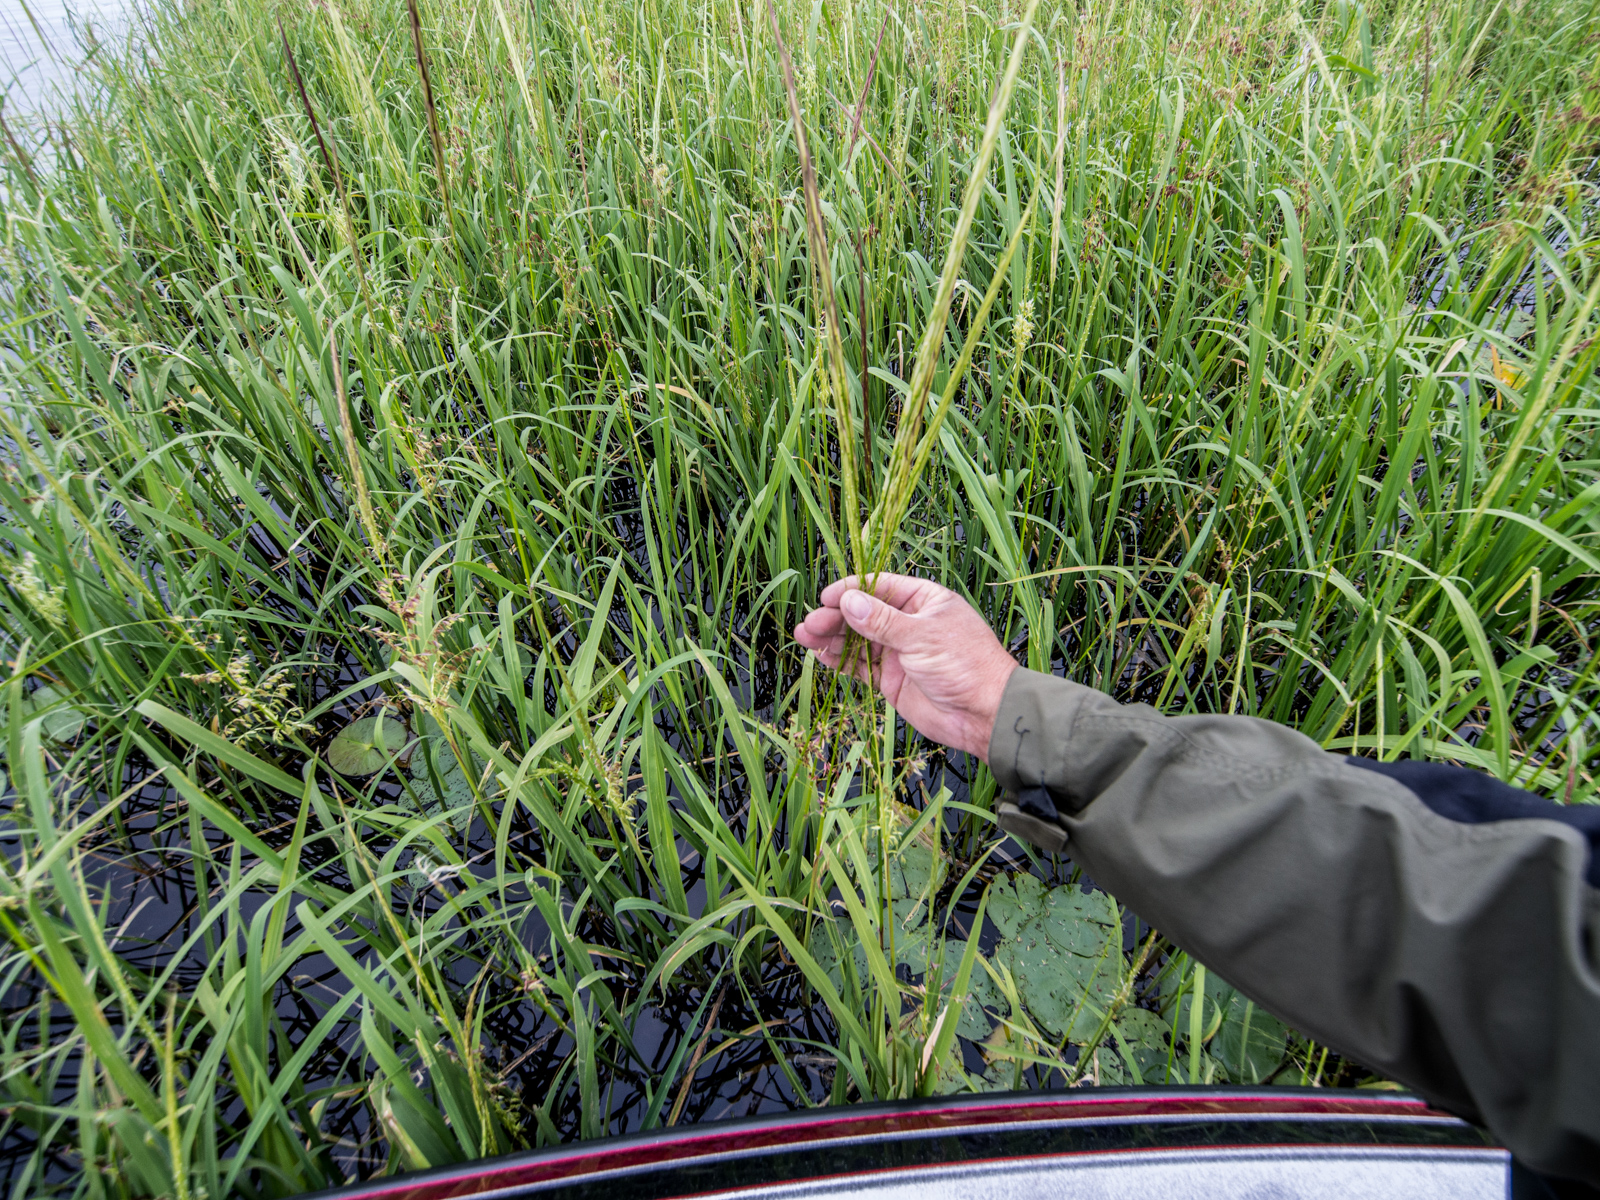
\includegraphics[height=\paperheight]{20150804_194209.jpg}}

\begin{frame}{Impact on 2015 Wild Rice Production}

\end{frame}
}

%%%%%%%%%1%%%%%%%%%2%%%%%%%%%3%%%%%%%%%4%%%%%%%%%5%%%%%%%%%6%%%%%%%%%7%%%%%%%%%8

{{\usebackgroundtemplate%
	{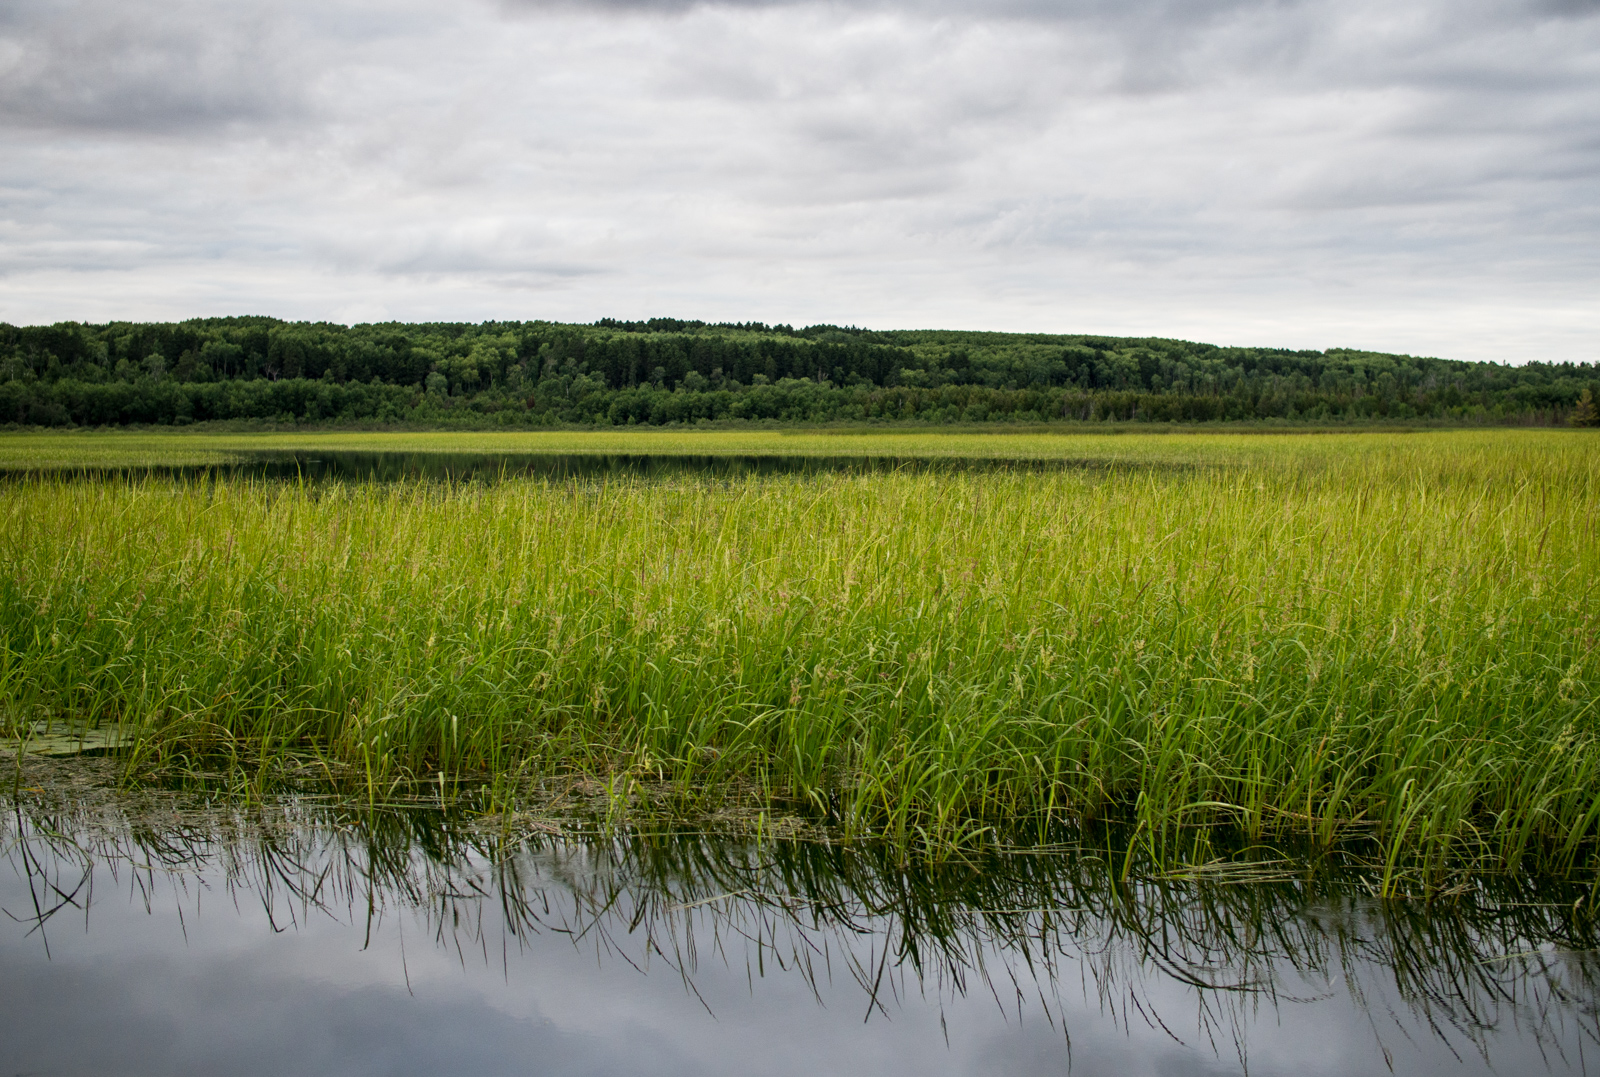
\includegraphics[height=\paperheight]{20150804_195914.jpg}}

\begin{frame}{}

\end{frame}
}

%%%%%%%%%1%%%%%%%%%2%%%%%%%%%3%%%%%%%%%4%%%%%%%%%5%%%%%%%%%6%%%%%%%%%7%%%%%%%%%8
% Section 
%%%%%%%%%1%%%%%%%%%2%%%%%%%%%3%%%%%%%%%4%%%%%%%%%5%%%%%%%%%6%%%%%%%%%7%%%%%%%%%8

{\usebackgroundtemplate%
	{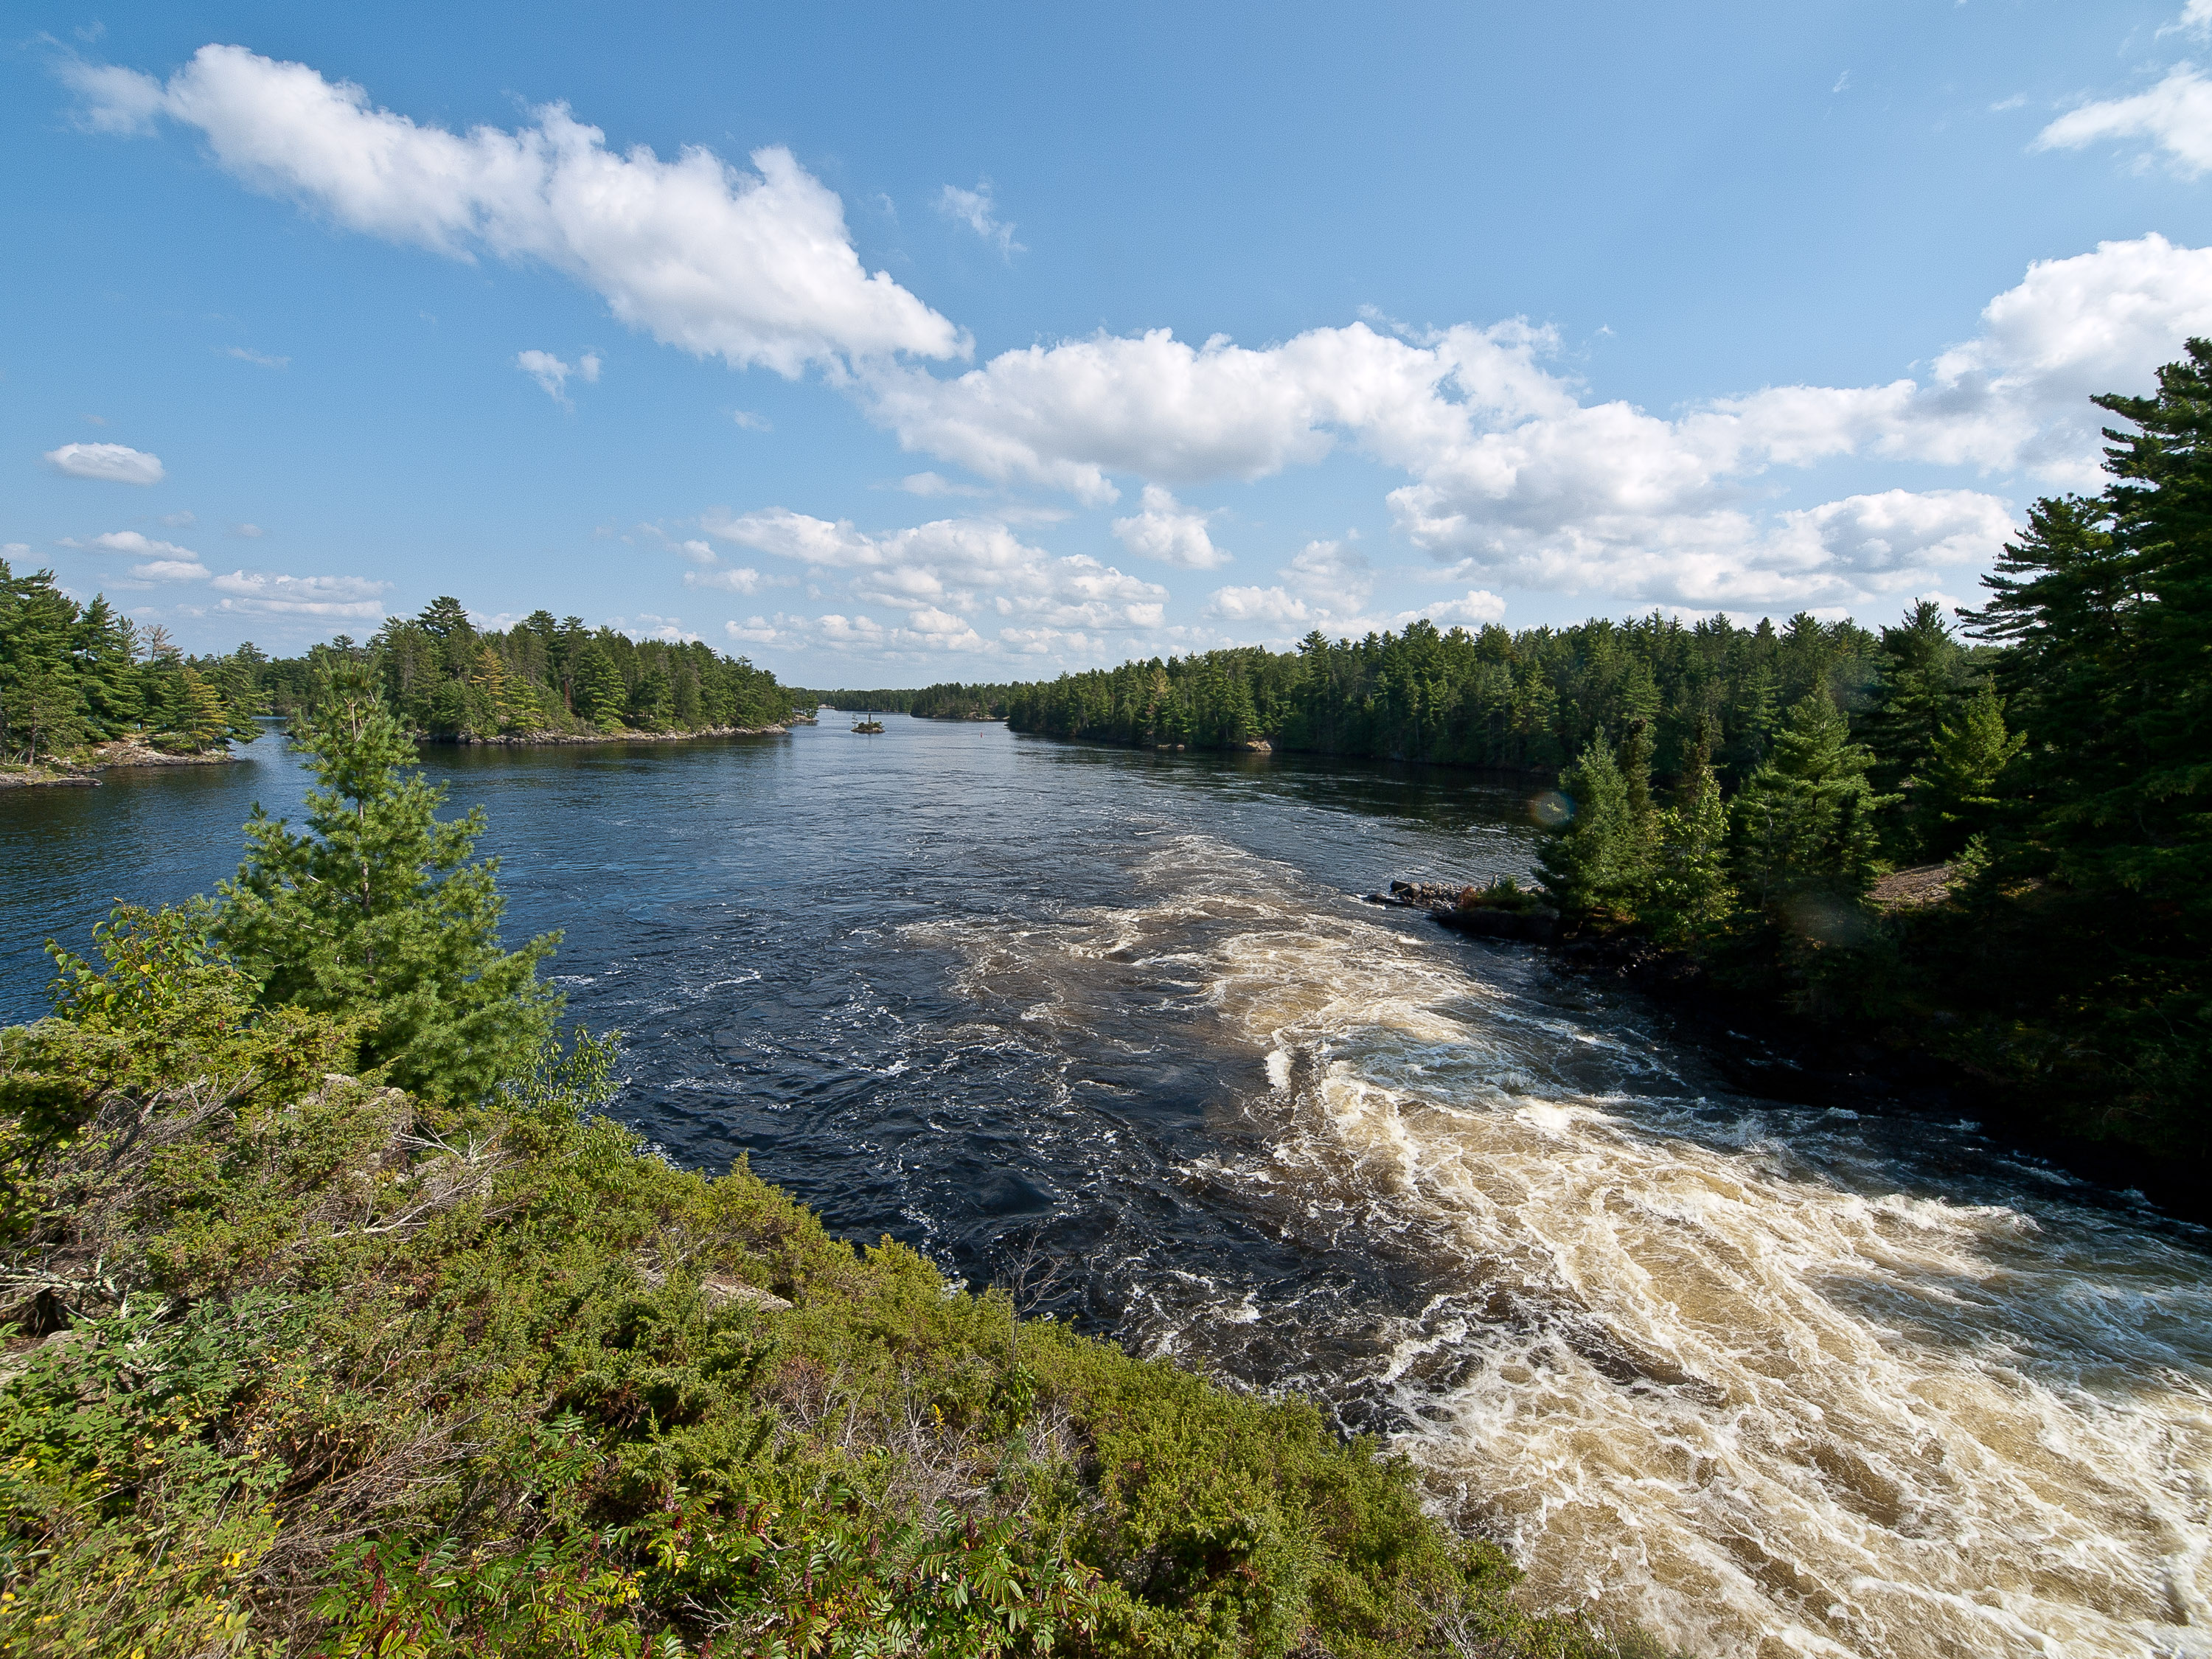
\includegraphics[height=\paperheight]{KettleChannel.jpg}}
\section{Implications for the Rule Curve Review}
}

%%%%%%%%%1%%%%%%%%%2%%%%%%%%%3%%%%%%%%%4%%%%%%%%%5%%%%%%%%%6%%%%%%%%%7%%%%%%%%%8
\begin{frame}{1993 Final Report and Recommendations}

"{\color{red}To offset the potential for the proposed rule curve modifications to increase the frequency of spring flood events}, the IJC should enforce the provision of its 1970 Supplemental Order {\color{red} requiring the dam operators to anticipate inflows and maximize the discharge capabilities of the dams to prevent emergency water levels}. 

"The Steering Committee believes that {\color{red} diligent use of the existing network of upstream lake level gauges and currently available hydrologic models can make this IJC mandate a reality and improve the accuracy and reliability of reservoir level control}." 

\vspace*{3mm}
\usebeamerfont{copyright text}{\usebeamercolor[fg]{copyright text}{Source: Rainy Lake \& Namakan Reservoir Water Level International Steering Committee, Final Report and Recommendations, November, 1993.}}

\end{frame}


%%%%%%%%%1%%%%%%%%%2%%%%%%%%%3%%%%%%%%%4%%%%%%%%%5%%%%%%%%%6%%%%%%%%%7%%%%%%%%%8
\begin{frame}{Conclusions}

{\bf The rule curve review needs to include control implementation within the scope of its work.}

\begin{enumerate}

\item Contrary to the 1993 Report, there is little evidence for "diligent use of existing network of upstream lake level gauges and currently available hydrological models can make this IJC mandate a reality and improve the accuracy and reliability of reservoir level control."

\item The 2000 rule curves are not a feasible mandate for level management on Rainy Lake.

\item  Consideration should be given to an integrated control strategy for flow control points on the Rainy-Lake of the Woods watershed coupled with significant rule curve revisions.
	
\end{enumerate}

\end{frame}

%%%%%%%%%1%%%%%%%%%2%%%%%%%%%3%%%%%%%%%4%%%%%%%%%5%%%%%%%%%6%%%%%%%%%7%%%%%%%%%8
% Section 
%%%%%%%%%1%%%%%%%%%2%%%%%%%%%3%%%%%%%%%4%%%%%%%%%5%%%%%%%%%6%%%%%%%%%7%%%%%%%%%8

{\usebackgroundtemplate%
	{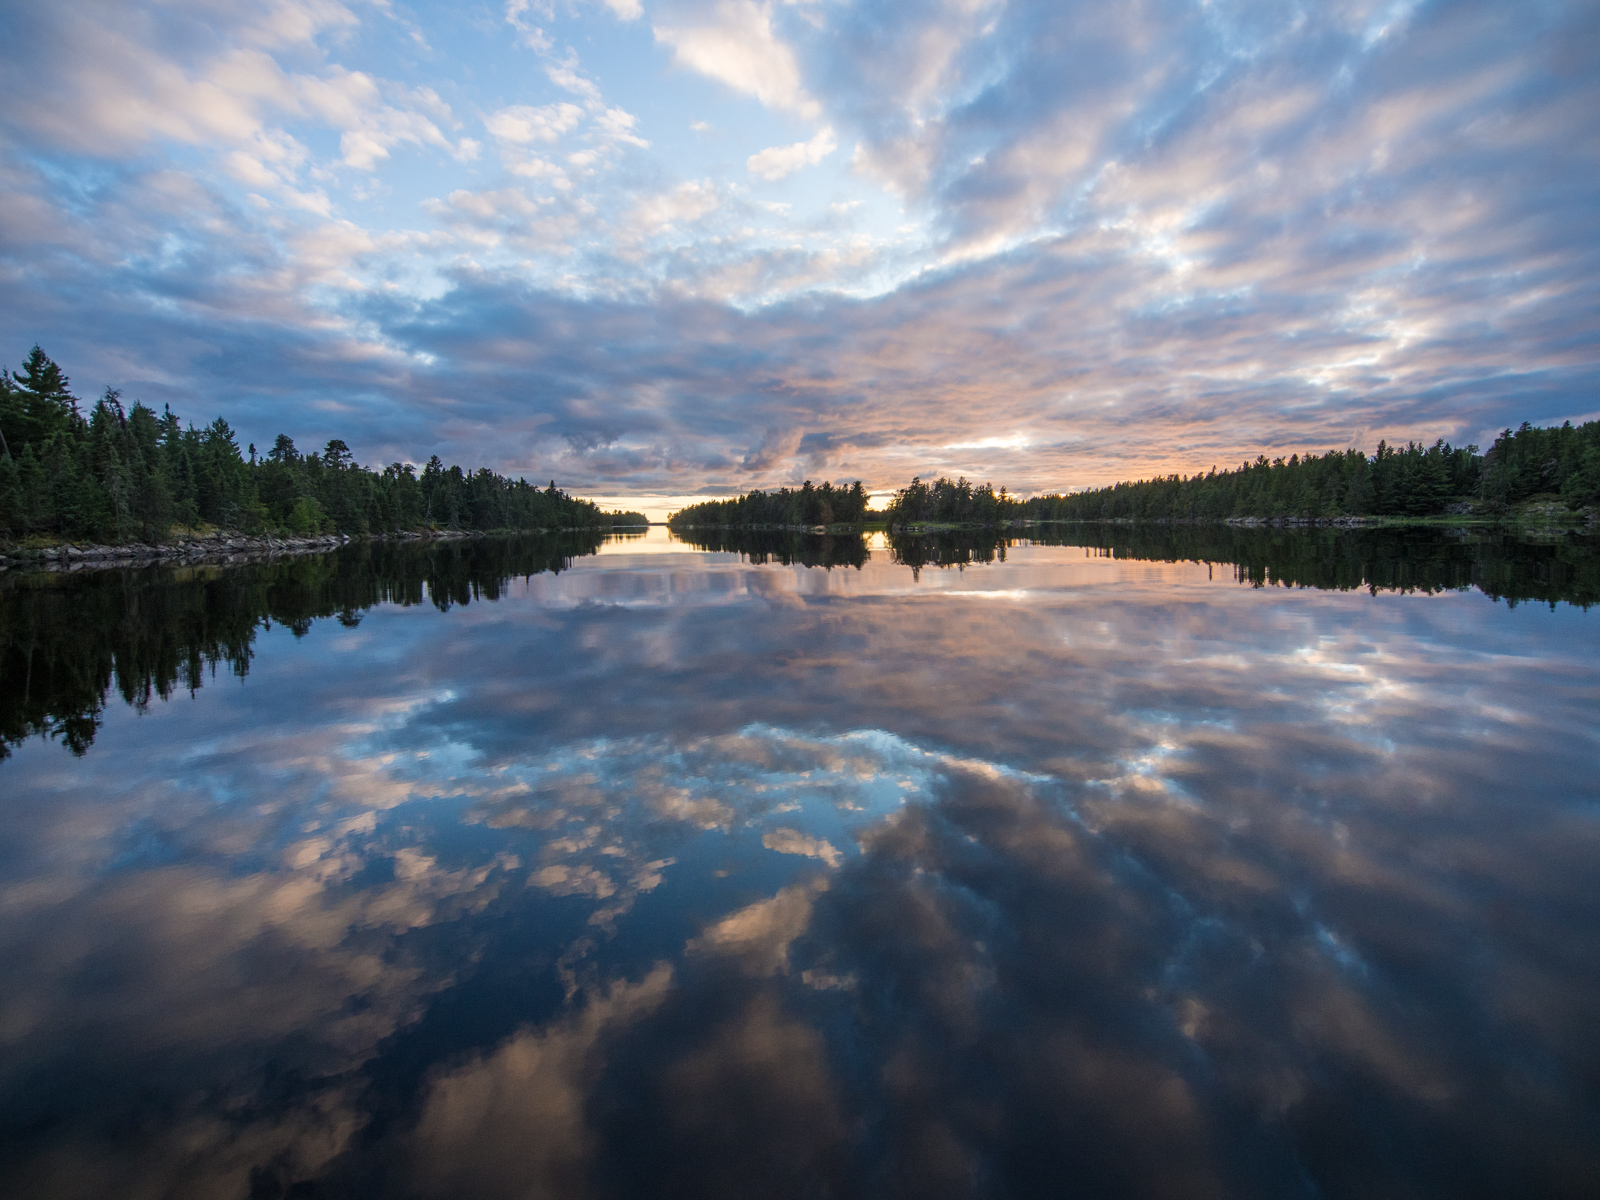
\includegraphics[width=\paperwidth]{20150804_202405.jpg}}
	
\begin{frame}{}

\vfill\vfill
\begin{center}
{\LARGE\color{white}{Research Projects}}
\end{center}

\end{frame}
}

%%%%%%%%%1%%%%%%%%%2%%%%%%%%%3%%%%%%%%%4%%%%%%%%%5%%%%%%%%%6%%%%%%%%%7%%%%%%%%%8
\begin{frame}{Research Objective}

The main focus of this work is to provide insight into the challenges and opportunities for control of water levels on a prototypical lake system in the Canadian Shield. 

\end{frame}


%%%%%%%%%1%%%%%%%%%2%%%%%%%%%3%%%%%%%%%4%%%%%%%%%5%%%%%%%%%6%%%%%%%%%7%%%%%%%%%8
\begin{frame}{Advanced Control for Rainy and Namakan Lake Levels}

{\bf Develop multivariable MPC model for the control of Rainy Lake. Develop historical comparisons and tune on a training set. Demonstrate relative performance for select years.}

\begin{enumerate}

\item Fully implement the 2000 Rule Curve order, with a facility to explore changes to essential components. Implement, train, and test
\begin{enumerate}
\item Baseline control to the median of the rule curve.
\item Control to other quantiles of the rule curve.
\item Multiloop PID control.
\item Implement MPC control.
\item Implement Stochastic MPC.	
\end{enumerate}
\item Develop a recommended control strategy for testing and implementation by the IJC.
\end{enumerate}

Would the proposed controls have had a beneficial impact during the 2014 flooding events?


\end{frame}

%%%%%%%%%1%%%%%%%%%2%%%%%%%%%3%%%%%%%%%4%%%%%%%%%5%%%%%%%%%6%%%%%%%%%7%%%%%%%%%8
\begin{frame}{Dynamics and Control of Seine River Watershed}

{\bf Develop a Matlab/Simulink and Python models for the reservoirs and dams on the Seine River, and test against historical data.  Develop RHC control options for the regulation of flows and levels.}

\begin{enumerate}

\item 
	
\end{enumerate}

\end{frame}

%%%%%%%%%1%%%%%%%%%2%%%%%%%%%3%%%%%%%%%4%%%%%%%%%5%%%%%%%%%6%%%%%%%%%7%%%%%%%%%8
\begin{frame}{Predict Freshet}

{\bf Use Water Year data and weather inputs. Develop training and evaluation data sets.}

\begin{enumerate}

\item 
	
\end{enumerate}

\end{frame}

%%%%%%%%%1%%%%%%%%%2%%%%%%%%%3%%%%%%%%%4%%%%%%%%%5%%%%%%%%%6%%%%%%%%%7%%%%%%%%%8
\begin{frame}{Rule Curve Design by Multiobjective Optimization}

{\bf Review existing methodologies for rule curve design, and apply to the Rainy Lake/Namakan System.}

\begin{enumerate}

\item 
	
\end{enumerate}

\end{frame}



%%%%%%%%%1%%%%%%%%%2%%%%%%%%%3%%%%%%%%%4%%%%%%%%%5%%%%%%%%%6%%%%%%%%%7%%%%%%%%%8
\begin{frame}{Acknowledgements}
\begin{small}
\begin{itemize}
\item Emmy Popovich, UG research assistant
\item Nicole Mejias, UG research assistant
\item \href{http://engineering.nd.edu/profiles/ahamlet/}{Alan Hamlet}, CEEES, Notre Dame
\item Aaron Thompson, Directorate Environment Canada
\item RLPOA Research and Technology Committee:
\begin{multicols}{3}
\begin{itemize}
\item Tom Dougherty
\item Jim Yount
\item Bruce Walker
\item Howard Hansen
\item Tom Biondich
\item Kirk Skallman
\item Geo. Simmons
\item Tom Smith
\item Mike Williams
\item Jim Giauque
\item Mark Gagnier
\item Paul Anderson
\item Jason Lindquist
\item Eric Olson
\item Scott Klosner
\end{itemize}
\end{multicols}
\end{itemize}
\end{small}

\begin{footnotesize}
The content of this presentation is the independent work product of the author conducted in compliance with policies on research and outside activities at the University of Notre Dame. No financial support has been received from any source.
\end{footnotesize}

\end{frame}

%%%%%%%%%1%%%%%%%%%2%%%%%%%%%3%%%%%%%%%4%%%%%%%%%5%%%%%%%%%6%%%%%%%%%7%%%%%%%%%8
\begin{frame}{Additional Photo Credits}

\begin{center}
\begin{tabular}{cp{3cm}p{0.3cm}cp{3cm} }
\raisebox{-0.5\height}{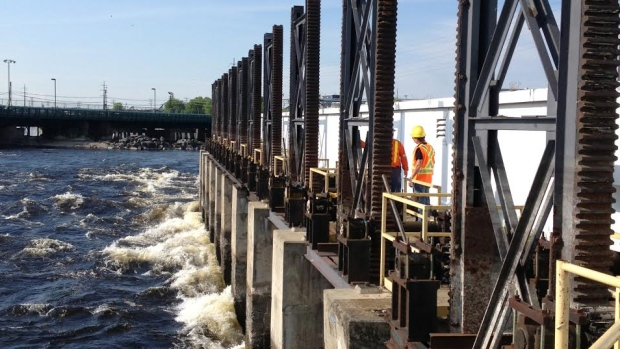
\includegraphics[height=1cm]{fort-frances-dam.jpg}} & Lee Grim - IJC
& & 
\raisebox{-0.5\height}{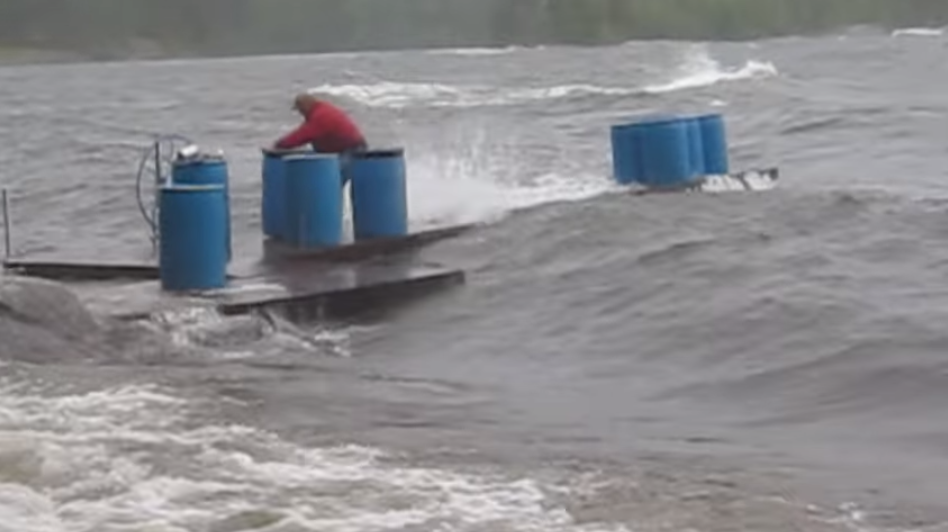
\includegraphics[height=1cm]{WaterBarrelsDock}} & Melody Hensel
\\ \\
\raisebox{-0.5\height}{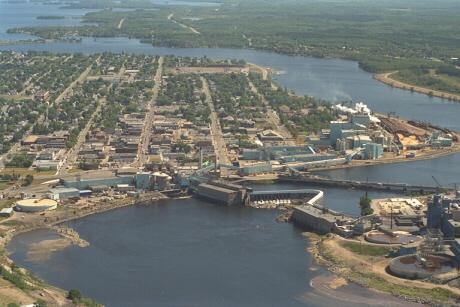
\includegraphics[height=1cm]{mill.jpg}} & Mike's Fly In
& &
\raisebox{-0.5\height}{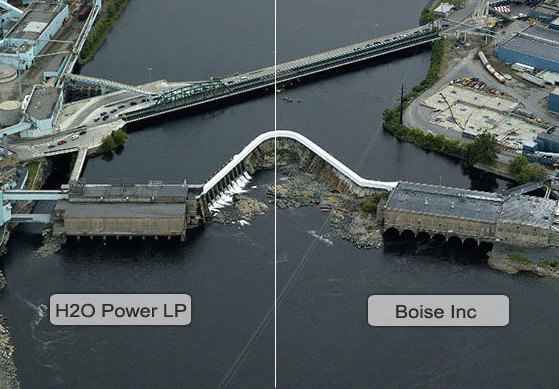
\includegraphics[height=1cm]{fort-frances-split.jpg}} & h2opower.ca
\end{tabular}
\end{center}


\end{frame}

%%%%%%%%%1%%%%%%%%%2%%%%%%%%%3%%%%%%%%%4%%%%%%%%%5%%%%%%%%%6%%%%%%%%%7%%%%%%%%%8
% End of Document
%%%%%%%%%1%%%%%%%%%2%%%%%%%%%3%%%%%%%%%4%%%%%%%%%5%%%%%%%%%6%%%%%%%%%7%%%%%%%%%8

\end{document}

%%%%%%%%%1%%%%%%%%%2%%%%%%%%%3%%%%%%%%%4%%%%%%%%%5%%%%%%%%%6%%%%%%%%%7%%%%%%%%%8
% Unused Materials
%%%%%%%%%1%%%%%%%%%2%%%%%%%%%3%%%%%%%%%4%%%%%%%%%5%%%%%%%%%6%%%%%%%%%7%%%%%%%%%8

%%%%%%%%%1%%%%%%%%%2%%%%%%%%%3%%%%%%%%%4%%%%%%%%%5%%%%%%%%%6%%%%%%%%%7%%%%%%%%%8
\begin{frame}{Control Points on Rainy Lake Watershed}

\begin{description}
\item [Calm Lake Generating Station] Run-of-river hydroelectric station on the Seine River operated under the Seine River Water Management Plan. 	
\end{description}

\begin{center}
	\begin{tabular}{lc}\toprule
Dam & Capacity \\
\midrule
Raft Lake Dame & \\

\end{tabular}
\end{center}
	
\end{frame}
